% =====================================================================
%  Rapport de PFE — fichier racine (root document)
%  Compilation : pdflatex (via latexmk dans LaTeX Workshop)
% =====================================================================

% Classe du document (charge la plupart des packages : voir pfe-report.cls)
\documentclass[12pt, oneside, a4paper]{pfe-report}

% --- Préambule -------------------------------------------------------
% Ordre important :
%   1) packages  : packages additionnels non fournis par la classe
%   2) Commands  : commandes personnalisées (\reportTitle, \reportAuthor, ...)
%   3) config    : métadonnées PDF (\hypersetup), minitoc, graphicspath
% \input (et NON \include) : on est dans le préambule, \include y est interdit.
% Packages additionnels pour le rapport de PFE.
%
% NOTE IMPORTANTE : la classe pfe-report.cls charge déjà babel(french), hyperref,
% caption/subcaption, tabularx, pdfpages, graphicx, ragged2e, xcolor, geometry, etc.
% On NE les recharge donc PAS ici (cela créerait des redondances / "Option clash").
% On ne déclare que les packages qui ne sont PAS déjà fournis par la classe.

\usepackage{amsmath}        % Formules mathématiques avancées
\usepackage{longtable}      % Tableaux sur plusieurs pages
\usepackage{hyphenat}       % Gestion fine des césures
\usepackage{utfsym}         % Symboles Unicode supplémentaires
\usepackage{float}          % Placement précis des flottants (option [H])

% Commandes personnalisées du rapport de PFE
% Ce fichier est chargé via % Commandes personnalisées du rapport de PFE
% Ce fichier est chargé via % Commandes personnalisées du rapport de PFE
% Ce fichier est chargé via \input{Commands} dans le préambule (PAS \include).

% --- Métadonnées utilisées par \hypersetup (config.tex) ---
\newcommand{\reportTitle}{Titre du Projet de Fin d'Études}
\newcommand{\reportSubject}{Rapport de Projet de Fin d'Études}
\newcommand{\reportAuthor}{Prénom \textsc{NOM}}

% --- Exemple de commande utilitaire ---
\newcommand{\MyCommand}{%
  Does nothing really%
}
 dans le préambule (PAS \include).

% --- Métadonnées utilisées par \hypersetup (config.tex) ---
\newcommand{\reportTitle}{Titre du Projet de Fin d'Études}
\newcommand{\reportSubject}{Rapport de Projet de Fin d'Études}
\newcommand{\reportAuthor}{Prénom \textsc{NOM}}

% --- Exemple de commande utilitaire ---
\newcommand{\MyCommand}{%
  Does nothing really%
}
 dans le préambule (PAS \include).

% --- Métadonnées utilisées par \hypersetup (config.tex) ---
\newcommand{\reportTitle}{Titre du Projet de Fin d'Études}
\newcommand{\reportSubject}{Rapport de Projet de Fin d'Études}
\newcommand{\reportAuthor}{Prénom \textsc{NOM}}

% --- Exemple de commande utilitaire ---
\newcommand{\MyCommand}{%
  Does nothing really%
}

% Custom configuration for the PFE Report

% Text justification throughout the document
\justifying

% PDF metadata configuration
\hypersetup{
  pdftitle={\reportTitle~-~\reportSubject},  % Titre du document
  pdfauthor={\reportAuthor},                % Auteur du document
  pdfsubject={\reportSubject},              % Sujet du rapport
  pdfkeywords={report} {internship} {pfe}
}

% Mini table of contents per chapter
\dominitoc

% Graphics path for images
\graphicspath{{images/}}


% =====================================================================
\begin{document}

    % Double interligne pour la lisibilité
    \doublespacing{}

    % Numérotation romaine pour les pages liminaires
    \pagenumbering{roman}

    % --- Pages liminaires --------------------------------------------
    \chapter*{DÉDICACES}
%\addstarredchapter{DEDICATION}
%\addcontentsline{toc}{chapter}{DEDICATION}
%\adjustmtc
\thispagestyle{MyStyle}

\begingroup
\itshape

\begin{center}
{\large\bfseries À la mémoire de ma très chère mère,}
\end{center}

\bigskip

Cette réalisation est avant tout dédiée à ma mère, qui nous a quittés après
un courageux combat contre le cancer. Son amour, sa bienveillance et les valeurs qu'elle
m'a transmises continuent de guider chacun de mes pas. Son souvenir restera à jamais gravé
dans mon c\oe ur, et je lui dédie ce travail avec une profonde émotion et une immense
reconnaissance.

Je dédie également ce projet à Dieu Tout-Puissant, qui m'a accordé la force, la patience et
la persévérance nécessaires pour surmonter les difficultés rencontrées tout au long de ce
parcours. C'est par Sa grâce que j'ai pu mener ce projet à son terme.

À mon père, Mohamed Salah Rebhi, je tiens à exprimer toute ma gratitude pour son soutien
indéfectible, ses sacrifices, ses encouragements et sa confiance permanente. Son amour et
son accompagnement ont été une source de motivation essentielle tout au long de mes études.

À mes s\oe urs, Nouha et Rahma, ainsi qu'à mon frère Moujahed, merci pour votre présence,
votre affection et vos encouragements constants. Votre soutien moral a été d'une valeur
inestimable dans les moments les plus exigeants de ce parcours.

Je souhaite également dédier ce travail à tous mes amis qui m'ont accompagné durant ces
années d'études et qui ont contribué, chacun à leur manière, à mon évolution personnelle et
professionnelle. Je pense tout particulièrement à Aymen Ferchichi, Malek Daoud et Zahra Elair,
dont les conseils, les échanges et l'entraide ont largement contribué au développement de
mes compétences.

Enfin, je tiens à adresser une pensée particulière aux amis et collègues que j'ai eu la
chance de rencontrer au sein de Talan Tunisie Consulting, et plus particulièrement de
l'équipe Innovation Factory. Leur esprit de collaboration, leur disponibilité, leur bonne
humeur et les nombreux échanges techniques ont rendu cette expérience humaine et
professionnelle particulièrement enrichissante.

À toutes les personnes qui ont cru en moi, soutenu mes efforts et contribué, de près ou de
loin, à la réalisation de ce projet, je dédie ce travail avec toute ma reconnaissance et mon
profond respect.

\bigskip

{\raggedleft\normalfont\large\itshape Ayoub Rebhi\par}

\endgroup
    % Dédicaces
    \chapter*{REMERCIEMENTS}
%\addstarredchapter{REMERCIEMENT}
%\addcontentsline{toc}{chapter}{REMERCIEMENT}
%\adjustmtc
\thispagestyle{MyStyle}

Avant toute chose, je tiens à remercier Dieu Tout-Puissant de m'avoir accordé la santé, la
force et la persévérance nécessaires pour mener à bien ce projet de fin d'études.

J'adresse mes plus sincères remerciements à mon encadrante académique à ESPRIT, Madame
Maroua Kssentini, pour la qualité de son enseignement, sa disponibilité, sa confiance ainsi
que ses précieux conseils. Son accompagnement et ses remarques pertinentes ont constitué un
soutien précieux tout au long de la réalisation de ce travail et de la rédaction de ce
rapport.

Je tiens également à exprimer ma profonde gratitude à mes encadrantes professionnelles,
Madame Emna Felfel et Madame Sarra Ben Massaoud, pour leur encadrement, leur disponibilité,
leur écoute et leurs conseils tout au long de mon stage. Leur expertise et leur confiance
m'ont permis d'évoluer dans un environnement stimulant et de mener ce projet dans les
meilleures conditions.

Mes sincères remerciements s'adressent également à l'ensemble des collaborateurs de Talan
Tunisie Consulting, et plus particulièrement à l'équipe Innovation Factory, pour leur
accueil chaleureux, leur esprit de partage et leur accompagnement. Cette expérience a
constitué une étape déterminante dans mon parcours, tant sur le plan technique que sur le
plan humain.

Je remercie également tous les enseignants d'ESPRIT qui ont contribué à ma formation durant
ces années d'études et qui m'ont permis d'acquérir les connaissances nécessaires à la
réalisation de ce projet.

Enfin, j'adresse mes plus vifs remerciements aux membres du jury qui ont accepté d'examiner
ce travail. Je les remercie sincèrement pour l'intérêt qu'ils lui portent ainsi que pour le
temps consacré à son évaluation et aux remarques qu'ils formuleront afin d'enrichir ce
travail.
  % Remerciements

    % --- Table des matières ------------------------------------------
    \addtocontents{toc}{\protect\thispagestyle{MyStyle}}
    \renewcommand*\contentsname{TABLE DES MATIÈRES}
    \begin{spacing}{1}
    \tableofcontents
    \end{spacing}

    % --- Liste des figures -------------------------------------------
    \addtocontents{lof}{\protect\thispagestyle{MyStyle}}
    \renewcommand{\listfigurename}{LISTE DES FIGURES}
    \begin{spacing}{1}
    \listoffigures
    \end{spacing}
    \addcontentsline{toc}{chapter}{\listfigurename}
    \adjustmtc

    % --- Liste des tableaux ------------------------------------------
    \addtocontents{lot}{\protect\thispagestyle{MyStyle}}  % lot (et non lof) pour les tableaux
    \renewcommand{\listtablename}{LISTE DES TABLEAUX}
    \begin{spacing}{1}
    \listoftables
    \end{spacing}
    \addcontentsline{toc}{chapter}{\listtablename}
    \adjustmtc

    % --- Sections introductives --------------------------------------
    \chapter*{LISTE DES ABRÉVIATIONS}
\markboth{\MakeUppercase{LISTE DES ABRÉVIATIONS}}{}
\addcontentsline{toc}{chapter}{LISTE DES ABRÉVIATIONS}
\adjustmtc
\thispagestyle{MyStyle}

\begin{acronym}
\acro{IA}{Intelligence Artificielle }




\end{acronym}        % Liste des abréviations
    \chapter*{Introduction Générale}
\markboth{\MakeUppercase{Introduction Générale}}{}
\addcontentsline{toc}{chapter}{Introduction Générale}
\adjustmtc
\thispagestyle{MyStyle}

En une dizaine d'années, la manière de bâtir et d'exploiter les logiciels a changé de
nature. Portés par le Cloud Computing et le DevOps, les projets ont quitté les serveurs
traditionnels au profit d'architectures \textit{cloud-native}, fondées sur la
conteneurisation, l'\textit{Infrastructure as Code} et les pipelines d'intégration et de
livraison continues (CI/CD). À la clé~: des livraisons plus rapides, une forte automatisation
et des environnements aisément reproductibles.

Cette évolution a son revers, car la complexité grimpe. Mettre une application en production
oblige à composer avec un large éventail d'outils~--- Docker, Kubernetes, Terraform,
fournisseurs cloud~--- et à trancher, étape après étape, quantité de choix techniques.
Architecture, dimensionnement des ressources, agencement des artefacts, pipelines~: le moindre
faux pas de conception retentit sur la fiabilité comme sur le coût de l'infrastructure.

L'intelligence artificielle générative et les grands modèles de langage (LLM) laissent
entrevoir une aide réelle, sans pour autant remplacer l'expertise humaine~: leur rôle est
d'assister, non de décider. Les assistants actuels restent pourtant partiels. Beaucoup se
limitent à produire des fragments de code ou des configurations isolés, sans vue d'ensemble
du projet~; rares sont ceux qui analysent un dépôt de bout en bout, proposent une architecture
cloud adaptée aux contraintes, préparent des artefacts cohérents, font valider les choix ou
corrigent finement les erreurs. Faute de mieux, l'ingénieur doit recoller lui-même des
morceaux épars, sans garantie de cohérence.

C'est à ce manque que s'attaque le présent travail, réalisé lors d'un stage de fin d'études
chez Talan Tunisie Consulting. Nous y présentons \textbf{MultiMindOps}, une plateforme
d'assistance IA destinée aux ingénieurs Cloud et DevOps. Plutôt que de livrer des fichiers
détachés les uns des autres, elle accompagne l'ingénieur du début à la fin~: analyse
automatique du projet, propositions d'architectures cloud, estimation des ressources,
génération des principaux artefacts DevOps et validation assistée des décisions. Le principe
directeur en est le \textit{Human-in-the-Loop}~: l'ingénieur garde la maîtrise des
orientations stratégiques et approuve chaque étape. La sécurité, quant à elle, n'y forme pas
une brique isolée mais une exigence de qualité transversale, présente autant dans les
artefacts produits que dans l'architecture de la plateforme.

\bigskip

\noindent La suite du document s'organise ainsi :

\begin{itemize}
    \item \textbf{Chapitre 1 --- Cadre général du projet~:} il campe l'organisme d'accueil,
    précise le contexte et la problématique, passe en revue les outils existants, avant
    d'exposer la solution retenue et la méthodologie de travail.

    \item \textbf{Chapitre 2 --- Concepts fondamentaux~:} il réunit l'état de l'art des
    notions mobilisées~: intelligence artificielle générative et LLM, systèmes multi-agents,
    RAG, Infrastructure as Code, conteneurisation et orchestration cloud.

    \item \textbf{Chapitre 3 --- Analyse et conception~:} il traite l'analyse des besoins,
    la modélisation de l'architecture d'ensemble, les diagrammes UML et la conception fine
    des agents et des workflows.

    \item \textbf{Chapitre 4 --- Réalisation et mise en œuvre~:} il rend compte de
    l'implémentation, du déploiement des agents IA, de la génération des artefacts DevOps,
    des interfaces utilisateur et d'une démonstration des fonctionnalités.
\end{itemize}

\bigskip

\noindent Une conclusion générale clôt l'ensemble~: elle fait le bilan des apports de ce
travail et esquisse les pistes d'évolution envisagées pour la plateforme.
% Introduction générale

    % Numérotation arabe pour le corps du document
    \pagenumbering{arabic}
    \doublespacing{}

    % --- Chapitres ---------------------------------------------------
    \chapter{Cadre général du projet}
\begin{spacing}{1.2}
\minitoc % Affiche la minitoc du chapitre
\thispagestyle{MyStyle}
\end{spacing}
\clearpage

\section{Introduction}
Ce premier chapitre vise à présenter le projet dans son cadre général en exposant
son contexte, sa problématique ainsi que les objectifs visés. Nous commençons par
présenter l'organisme d'accueil, ses domaines d'expertise et son environnement
technologique. Nous détaillons ensuite le contexte du projet, les limites des
approches existantes et la solution proposée pour répondre aux problématiques
identifiées. Enfin, nous présentons la méthodologie de développement adoptée pour la
réalisation de cette plateforme intelligente orientée Cloud, DevSecOps et
Intelligence Artificielle.

\section{Présentation de l'organisme d'accueil}

\begin{figure}[H]
    \centering
    
\includegraphics[width=0.35\textwidth]{images/Logo_Talan.png}
    \caption{Logo de Talan}
    \label{fig:logo-talan}
\end{figure}

Talan est un groupe international spécialisé dans le conseil en innovation, la
transformation digitale et les technologies avancées. Présent dans plusieurs pays,
le groupe accompagne ses clients dans la modernisation de leurs systèmes
d'information à travers des solutions innovantes intégrant le Cloud Computing, la
Data, l'Intelligence Artificielle et les pratiques DevOps. Grâce à une expertise
multidisciplinaire, l'entreprise participe à la réalisation de projets à forte
valeur technologique destinés à des clients nationaux et internationaux.

\subsection{Services et domaines d'expertise}
Talan Tunisie Consulting intervient dans plusieurs domaines technologiques tels que
le développement logiciel, l'architecture cloud, la cybersécurité, le Data
Engineering, l'Intelligence Artificielle et les pratiques DevSecOps. L'entreprise
propose également des services de transformation digitale, d'intégration de
solutions métiers et d'accompagnement dans l'automatisation des infrastructures
informatiques. Forte de son expertise dans les technologies modernes telles que le
Cloud Computing, Kubernetes, Terraform et les architectures distribuées, elle
contribue à la mise en place de solutions robustes, sécurisées et évolutives,
adaptées aux besoins des organisations.

\subsection{Clients et partenariats stratégiques}
Talan collabore avec de nombreuses entreprises et organisations opérant dans des
secteurs variés tels que la finance, les télécommunications, l'industrie, le
transport et les services numériques. Le groupe développe par ailleurs des
partenariats stratégiques avec des acteurs technologiques majeurs afin
d'accompagner ses clients dans l'adoption des technologies innovantes et des
solutions cloud modernes. Ces collaborations lui permettent de bénéficier d'un
environnement technologique avancé et de participer à des projets internationaux
exigeant un haut niveau d'expertise technique et organisationnelle.

\subsection{Bootcamp : Talan Innovation Factory}
Le bootcamp s'est déroulé au sein de la \textit{Talan Innovation Factory}, entité
dédiée à la recherche et au développement de solutions innovantes au sein de Talan
Tunisie Consulting. Ce programme intensif d'une durée de quatre semaines a constitué
la phase initiale du stage et visait à renforcer les compétences techniques des
participants dans les domaines du Cloud, de l'Intelligence Artificielle et de la
cybersécurité.

La première semaine a été consacrée aux fondamentaux de l'Intelligence
Artificielle, du \textit{Machine Learning} et du \textit{Deep Learning}, avec la
réalisation d'un projet complet couvrant la préparation des données, l'entraînement
des modèles et leur déploiement. La deuxième semaine s'est focalisée sur le
\textit{Natural Language Processing} (NLP) et les \textit{Large Language Models}
(LLM), en explorant les architectures modernes fondées sur les \textit{transformers}
et leurs cas d'usage.

La troisième semaine a introduit les concepts d'\textit{Agentic AI} à travers une
approche \textit{Blue/Red Team}, permettant de simuler des attaques adverses et
d'évaluer la robustesse des systèmes multi-agents, tout en intégrant les notions de
sécurité et d'observabilité. Enfin, la quatrième semaine a abordé les technologies
émergentes telles que la \textit{Blockchain} décentralisée et le \textit{Quantum
AI}, tout en renforçant les compétences collaboratives et la démarche
\textit{Security by Design}.

Ce bootcamp a joué un rôle fondamental dans la conception du projet, en fournissant
les bases techniques et conceptuelles nécessaires à la réalisation d'une plateforme
reposant sur l'orchestration multi-agents, l'automatisation DevSecOps et les
architectures cloud intelligentes.

\section{Présentation du projet}

\subsection{Contexte du projet}
Ce projet a été réalisé dans le cadre du stage de fin d'études en vue de l'obtention
du diplôme d'ingénieur en informatique à l'ESPRIT, durant l'année universitaire
2025--2026, au sein de Talan Tunisie Consulting. Il s'inscrit dans les domaines du
Cloud Computing, du DevSecOps et de l'Intelligence Artificielle, et a pour objectif
la conception et le développement d'une plateforme intelligente capable d'assister
automatiquement les utilisateurs dans la conception d'architectures cloud modernes.
Le projet vise à automatiser l'analyse des projets logiciels, la génération des
artefacts \textit{Infrastructure as Code}, l'estimation des coûts cloud ainsi que la
détection et la correction intelligente des erreurs liées aux environnements DevOps
et Kubernetes.

\subsection{Énoncé du problème}
Dans le contexte actuel de transformation numérique accélérée, les entreprises
adoptent de plus en plus des architectures \textit{cloud-native} et des pratiques
DevSecOps afin d'améliorer la scalabilité, la performance et la rapidité de
déploiement de leurs applications. Cette évolution introduit toutefois une
complexité importante dans la conception et la gestion des infrastructures modernes,
notamment du fait de la multiplication des outils et technologies tels que Docker,
Kubernetes, Terraform et les pipelines CI/CD.

Les principaux défis identifiés sont les suivants :

\begin{itemize}
    \item \textbf{Complexité technologique élevée :} les équipes doivent maîtriser
    simultanément plusieurs outils et langages d'infrastructure (Dockerfile, YAML
    Kubernetes, Terraform HCL), ce qui accroît la charge cognitive et les risques
    d'erreurs.
    \item \textbf{Absence d'un processus unifié :} les étapes de conception,
    d'estimation des coûts et de déploiement sont souvent dissociées, entraînant un
    manque de cohérence globale dans l'architecture.
    \item \textbf{Erreurs fréquentes en environnement DevOps :} les configurations
    manuelles ou semi-automatisées génèrent des erreurs difficiles à diagnostiquer
    et à corriger, ce qui allonge le temps de mise en production.
    \item \textbf{Manque d'intelligence décisionnelle :} les outils existants ne
    fournissent pas de véritable aide à la décision pour comparer différentes
    architectures cloud selon le coût, les performances et la scalabilité.
    \item \textbf{Absence d'intégration FinOps :} l'estimation et l'optimisation des
    coûts cloud sont généralement traitées séparément du processus de conception
    technique.
    \item \textbf{Limites des solutions IA existantes :} les assistants fondés sur
    les LLM génèrent du code ou des configurations, mais sans garantie de cohérence
    globale ni mécanisme robuste de correction et de validation.
\end{itemize}

Ces limitations rendent difficile la conception rapide, fiable et optimisée
d'infrastructures cloud modernes, et font émerger un besoin fort d'une solution
intégrée, intelligente et orientée assistance architecturale.

\subsection{Objectifs du projet}
L'objectif principal de ce projet est de concevoir et de développer une plateforme
intelligente capable d'assister automatiquement les utilisateurs dans la conception
d'architectures cloud modernes et sécurisées. La solution vise à analyser les
projets logiciels, à proposer plusieurs stratégies d'infrastructure adaptées, à
estimer les coûts cloud et à générer automatiquement les artefacts DevSecOps
nécessaires (Docker, Terraform, Kubernetes et CI/CD). Le projet a également pour
objectif d'intégrer un mécanisme intelligent de détection et de correction des
erreurs afin d'améliorer la fiabilité des déploiements et de réduire les
interventions manuelles dans les environnements \textit{cloud-native}.

\subsection{Analyse des approches existantes}
Avec l'évolution des technologies Cloud, DevOps et Intelligence Artificielle,
plusieurs plateformes et outils ont émergé afin d'automatiser certaines tâches liées
à la gestion d'infrastructure, à la génération d'artefacts DevOps et à l'assistance
au développement logiciel. Cependant, la majorité de ces solutions restent limitées
à des fonctionnalités spécifiques et ne proposent pas une approche globale combinant
l'analyse de code, l'aide à la décision architecturale, l'estimation des coûts, la
génération \textit{Infrastructure as Code} et la correction intelligente des
erreurs.

\subsubsection{Harness (AIDA)}

\begin{figure}[H]
    \centering
    
\includegraphics[width=0.30\textwidth]{images/logo_harness.png}
    \caption{Logo de Harness}
    \label{fig:logo-harness}
\end{figure}

Harness est une plateforme spécialisée dans les pipelines CI/CD et l'automatisation
du cycle de livraison logicielle. Elle intègre un assistant IA, baptisé AIDA,
capable d'analyser les pipelines, de prédire certains échecs et de proposer des
correctifs automatiques. Cette solution partage plusieurs objectifs avec notre
projet, notamment l'analyse intelligente des erreurs et l'automatisation DevSecOps.
Néanmoins, Harness demeure fortement dépendante de son propre écosystème CI/CD et
offre une flexibilité limitée pour l'analyse complète de dépôts GitHub et la
génération d'architectures cloud personnalisées.

\subsubsection{Pulumi Insights}

\begin{figure}[H]
    \centering
    
\includegraphics[width=0.30\textwidth]{images/Logo_pulumi_insights.png}
    \caption{Logo de Pulumi Insights}
    \label{fig:logo-pulumi}
\end{figure}

Pulumi propose une solution orientée \textit{Infrastructure as Code} permettant de
générer et de gérer des infrastructures cloud à l'aide de langages de programmation
modernes. Avec Pulumi Insights, la plateforme introduit des fonctionnalités
d'intelligence cloud permettant d'interroger l'infrastructure en langage naturel et
de générer automatiquement des configurations. Cette approche se rapproche de notre
\textit{Infrastructure Agent}. Toutefois, Pulumi ne réalise pas d'analyse
approfondie du code source applicatif afin de déduire automatiquement l'architecture
cloud adaptée, ce qui limite son niveau d'automatisation décisionnelle.

\subsubsection{Claude Code (Anthropic)}

\begin{figure}[H]
    \centering
    
\includegraphics[width=0.30\textwidth]{images/Logo_Claude_Code.png}
    \caption{Logo de Claude Code}
    \label{fig:logo-claude-code}
\end{figure}

Anthropic a récemment introduit Claude Code, un assistant agentique fonctionnant en
ligne de commande et capable d'analyser un dépôt local, d'en comprendre la structure
et de proposer des modifications de code ou de configuration. Cette solution présente
des similarités avec notre \textit{CodebaseAnalysisAgent} grâce à sa capacité
d'analyse contextuelle des projets logiciels. Cependant, Claude Code reste
principalement orienté assistance au développeur et ne propose ni architecture
multi-agents spécialisée, ni workflow DevSecOps structuré, ni système complet d'aide
à la décision cloud et de validation multi-étapes.

\subsection{Évaluation critique des systèmes existants}
Afin d'évaluer les limites des solutions actuelles et de positionner notre
plateforme par rapport aux approches existantes, nous avons réalisé une étude
comparative fondée sur plusieurs critères techniques et fonctionnels. Cette analyse,
synthétisée dans le tableau~\ref{tab:comparaison-solutions}, met en évidence les
différences entre les plateformes orientées DevSecOps / \textit{Infrastructure as
Code} et notre approche reposant sur une architecture multi-agents intelligente
intégrant l'analyse contextuelle, l'aide à la décision cloud et la correction
automatique des erreurs.

\begin{table}[H]
    \centering
    \footnotesize
    \begin{tabularx}{\textwidth}{|>{\raggedright\arraybackslash}p{3.2cm}|>{\raggedright\arraybackslash}X|>{\raggedright\arraybackslash}X|>{\raggedright\arraybackslash}X|>{\raggedright\arraybackslash}X|}
        \hline
        \rowcolor{tableRow1}
        \textbf{Critère} & \textbf{Harness AIDA} & \textbf{Pulumi Insights} & \textbf{Claude Code} & \textbf{Notre plateforme} \\
        \hline
        Interface utilisateur avancée & Interface CI/CD intégrée & Interface orientée IaC & Interface terminal CLI & Dashboard React interactif + monitoring temps réel \\
        \hline
        Génération Infrastructure as Code & Partielle & Oui & Partielle & Oui (Docker, Terraform, Kubernetes, CI/CD) \\
        \hline
        Analyse sémantique du code source & Limitée & Non & Partielle & Oui \\
        \hline
        Correction automatique des erreurs & Partielle & Non & Limitée & Oui \\
        \hline
        Automatisation du workflow DevSecOps & Moyenne & Moyenne & Faible & Élevée \\
        \hline
        Estimation et optimisation des coûts cloud & Limitée & Partielle & Non & Oui \\
        \hline
        Architecture multi-agents IA & Non & Non & Partielle & Oui \\
        \hline
        Validation humaine multi-étapes & Limitée & Non & Non & Oui \\
        \hline
        Analyse des logs et remédiation intelligente & Partielle & Non & Non & Oui \\
        \hline
        Flexibilité vis-à-vis des projets GitHub & Moyenne & Moyenne & Élevée & Élevée \\
        \hline
    \end{tabularx}
    \caption{Comparaison des solutions étudiées sur les critères clés du projet}
    \label{tab:comparaison-solutions}
\end{table}

Cette étude comparative montre que les solutions existantes répondent généralement à
des besoins spécifiques tels que l'automatisation CI/CD, la génération
\textit{Infrastructure as Code} ou l'assistance au développement logiciel. Elles ne
proposent toutefois pas une approche globale capable de combiner simultanément
l'analyse intelligente du projet, la prise de décision cloud, l'automatisation
DevSecOps, l'estimation des coûts et la correction intelligente des erreurs. Notre
plateforme cherche ainsi à combler ces limitations à travers une architecture
unifiée orientée assistance architecturale intelligente.

\subsection{Solution proposée}
Afin de répondre aux limitations des solutions existantes, nous proposons une
plateforme intelligente orientée Cloud Computing, DevSecOps et Intelligence
Artificielle, capable d'agir comme un véritable assistant d'architecture cloud. La
solution a pour objectif d'automatiser les différentes étapes de conception,
d'analyse et de préparation d'une infrastructure cloud moderne, tout en intégrant
des mécanismes avancés de validation, de correction et d'aide à la décision. Elle
repose principalement sur les éléments suivants :

\begin{itemize}
    \item \textbf{Architecture multi-agents IA :} plusieurs agents spécialisés
    collaborent pour analyser les projets, générer les artefacts et superviser les
    workflows DevSecOps.
    \item \textbf{Analyse intelligente du code source :} détection automatique des
    frameworks, dépendances, technologies et besoins infrastructurels à partir du
    dépôt GitHub fourni par l'utilisateur.
    \item \textbf{Système d'aide à la décision cloud :} génération de plusieurs
    stratégies d'architecture (\textit{Low Cost}, \textit{Balanced}, \textit{High
    Performance}) avec comparaison des coûts, des performances et des niveaux de
    scalabilité.
    \item \textbf{Génération automatique des artefacts IaC :} création automatisée
    des fichiers Docker, Terraform, Kubernetes et des pipelines CI/CD.
    \item \textbf{Structured Constrained Generation :} approche fondée sur des
    \textit{blueprints} YAML, une génération par sections et un assemblage
    déterministe afin de réduire les hallucinations des modèles IA.
    \item \textbf{RAG spécialisé par contexte technique :} système
    \textit{Section-Aware RAG} enrichissant chaque génération avec des bonnes
    pratiques spécifiques (sécurité Docker, Kubernetes, Terraform, optimisation
    cloud, etc.).
    \item \textbf{Correction intelligente des erreurs :} \textit{Corrector Agent}
    capable d'analyser les logs Docker, Terraform et Kubernetes, d'identifier les
    causes racines et de proposer des correctifs automatiques.
    \item \textbf{Architecture multi-LLM résiliente :} utilisation de GPT-5-mini
    comme modèle principal avec un mécanisme de \textit{fallback} automatique vers
    Groq afin d'assurer la continuité des services IA.
    \item \textbf{Monitoring temps réel :} affichage des logs d'exécution, des états
    des workflows et des processus de remédiation grâce aux WebSockets et à une
    interface React interactive.
    \item \textbf{Validation humaine multi-étapes :} points de validation permettant
    à l'utilisateur de contrôler et d'approuver les décisions critiques avant
    génération ou déploiement.
\end{itemize}

Cette solution vise ainsi à transformer les approches traditionnelles de gestion
d'infrastructure en une plateforme intelligente, automatisée et orientée assistance
architecturale avancée.

\section{Méthodologie de travail}
Afin de gérer efficacement le développement de ce projet complexe reposant sur
l'Intelligence Artificielle, le Cloud Computing et le DevSecOps, une approche
flexible et continue s'est avérée nécessaire. Compte tenu de l'évolution progressive
des besoins et des ajustements fréquents de l'architecture, la méthodologie Kanban a
été adoptée afin d'assurer une gestion fluide des tâches et une visibilité globale
sur l'avancement du projet.

\subsection{Étude comparative des méthodologies}
Le tableau~\ref{tab:comparaison-methodologies} présente une comparaison des
principales méthodologies de gestion de projet envisagées, au regard du contexte
spécifique de ce travail.

\begin{table}[H]
    \centering
    \footnotesize
    \begin{tabularx}{\textwidth}{|>{\raggedright\arraybackslash}p{3cm}|>{\raggedright\arraybackslash}X|>{\raggedright\arraybackslash}X|}
        \hline
        \rowcolor{tableRow1}
        \textbf{Méthodologie} & \textbf{Forces} & \textbf{Limites selon le contexte du projet} \\
        \hline
        Scrum &
        Organisation structurée en sprints \newline Bonne planification des livrables \newline Suivi régulier des objectifs &
        Moins flexible face aux changements rapides \newline Rigidité des cycles temporels \newline Difficulté d'adaptation aux ajustements continus \\
        \hline
        Kanban &
        Flux continu et flexible \newline Adaptation rapide aux changements \newline Visualisation claire de l'état des tâches \newline Limitation du travail en cours (WIP) &
        Moins de structure temporelle fixe \newline Moins adapté aux livrables strictement planifiés \\
        \hline
        Itératif \& Incrémental &
        Développement progressif \newline Amélioration continue du système \newline Réduction des risques techniques &
        Manque de visibilité globale du projet \newline Coordination complexe entre modules \\
        \hline
    \end{tabularx}
    \caption{Étude comparative des méthodologies de gestion de projet}
    \label{tab:comparaison-methodologies}
\end{table}

\subsection{Choix de Kanban pour le projet}
Le choix de la méthodologie Kanban a été motivé par plusieurs facteurs liés à la
nature évolutive du projet :

\begin{itemize}
    \item \textbf{Adaptation aux changements fréquents :} le projet a connu
    plusieurs évolutions architecturales importantes (multi-agents, Corrector Agent,
    Structured Constrained Generation), nécessitant une méthode capable de s'adapter
    en continu sans contrainte de sprint fixe.
    \item \textbf{Flux de développement continu :} Kanban autorise un avancement
    progressif des tâches, ce qui correspond à la nature expérimentale et itérative
    des composants IA et DevSecOps du système.
    \item \textbf{Visibilité et contrôle du travail en cours :} la gestion via un
    tableau Kanban a permis de suivre en temps réel l'état des tâches
    (\textit{Backlog}, \textit{In Progress}, \textit{Review}, \textit{Done}) et de
    limiter le travail simultané sur plusieurs modules complexes.
    \item \textbf{Gestion efficace des priorités techniques :} certaines
    fonctionnalités critiques (agents IA, correction automatique, génération IaC)
    ont nécessité des ajustements rapides de priorité, ce que Kanban facilite
    naturellement sans replanification globale.
\end{itemize}

\subsection{Planning du projet en Kanban}
Le projet s'est déroulé sur une période de six mois, du 2 février au 2 août 2026. Il
a débuté par un bootcamp de formation d'un mois permettant la montée en compétences
sur les technologies Cloud, DevSecOps et Intelligence Artificielle. Par la suite, le
développement a été géré selon une approche Kanban, où les tâches ont été
continuellement ajoutées, priorisées et exécutées en fonction de leur criticité et
de leurs dépendances techniques. Cette organisation a permis d'intégrer
progressivement les différentes évolutions architecturales du système, notamment la
mise en place de l'orchestration multi-agents, du moteur de décision cloud et du
système de correction automatique.

\subsection{Diagramme de Gantt}

\begin{figure}[H]
    \centering
    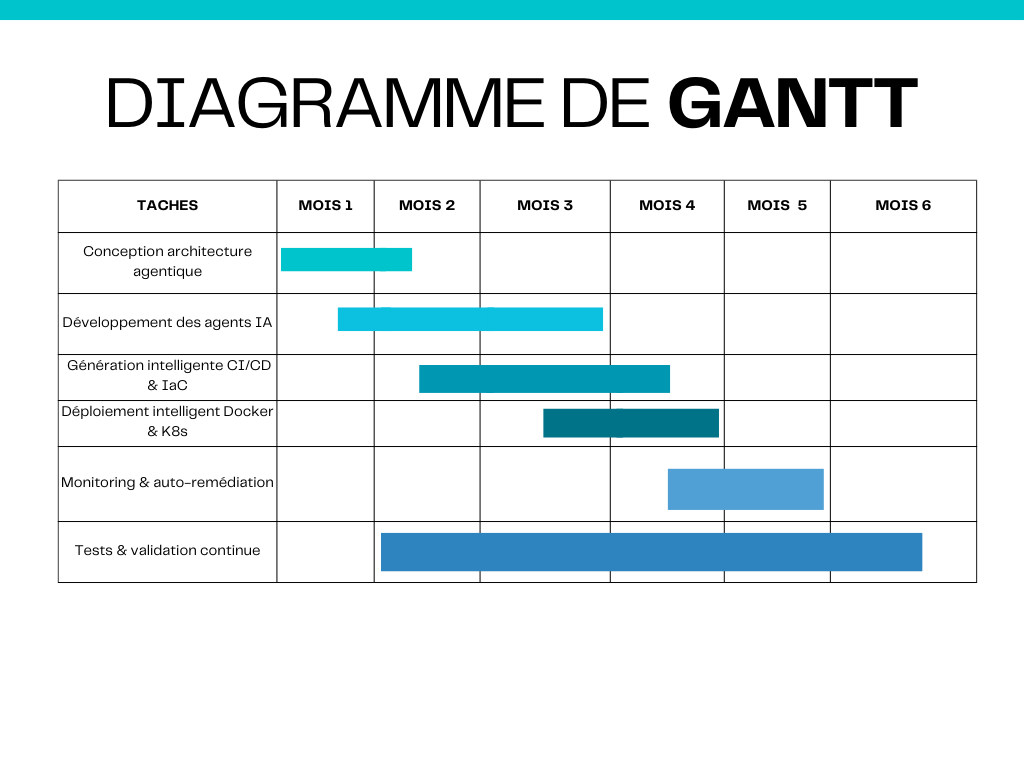
\includegraphics[width=0.95\textwidth]{images/Diag. GANTT.png}
    \caption{Planning du projet sur six mois (février $\rightarrow$ août 2026)}
    \label{fig:diagramme-gantt}
\end{figure}

\section{Conclusion}
Dans ce premier chapitre, nous avons présenté le cadre général du projet ainsi que
le contexte dans lequel il a été réalisé au sein de Talan Tunisie Consulting. Nous
avons exposé la problématique liée à la complexité des environnements Cloud et
DevSecOps modernes, ainsi que les limites des solutions existantes. Nous avons
ensuite décrit la solution proposée, puis la méthodologie Kanban adoptée pour la
gestion du projet. Le chapitre
suivant sera consacré à l'analyse et à la conception de la plateforme, en détaillant
l'architecture globale du système, les différents agents IA ainsi que les
technologies et mécanismes mis en \oe uvre pour la réalisation de la solution
proposée.

    \chapter{Concepts Fondamentaux}
\begin{spacing}{1.2}
\minitoc
\thispagestyle{MyStyle}
\end{spacing}
\clearpage

\section{Introduction}

Ce chapitre a pour objectif de présenter les concepts techniques qui constituent la
base de compréhension du projet. Avant d'aborder l'architecture et l'implémentation
de la plateforme, il est nécessaire de clarifier les notions fondamentales sur
lesquelles elle repose~: le DevSecOps, le Cloud Computing, l'Infrastructure as Code,
les pipelines CI/CD, la conteneurisation, et l'intégration de l'intelligence
artificielle dans les environnements d'automatisation. Ces concepts ne sont pas
simplement des buzzwords~; ils définissent concrètement la manière dont les systèmes
logiciels modernes sont construits et exploités.

\section{DevSecOps : culture et pratiques}

\subsection{Origines et définition}

Le terme DevSecOps est issu de la fusion de trois disciplines~: le développement
logiciel (\textit{Dev}), les opérations système (\textit{Ops}), et la sécurité
(\textit{Sec}). Il représente une évolution naturelle du mouvement DevOps apparu dans
les années 2010, dont l'objectif était de rapprocher les équipes de développement et
d'exploitation pour accélérer les cycles de livraison. L'ajout de la sécurité comme
composante native~--- plutôt que comme une étape finale de validation~--- est ce qui
définit le DevSecOps.

Concrètement, l'idée est d'intégrer les contrôles de sécurité directement dans le
pipeline de développement et de déploiement, à chaque étape, plutôt que de traiter
la sécurité comme une phase distincte. On parle de \textit{shift-left}~: les
vérifications de vulnérabilités, les analyses de code statique et les tests de
conformité sont effectués le plus tôt possible dans le cycle de vie logiciel.

\subsection{Principes clés}

Plusieurs principes structurent les pratiques DevSecOps. Le premier est
l'\textbf{automatisation}~: les contrôles manuels ne peuvent pas suivre la cadence
des déploiements continus. Il faut donc automatiser les tests, les scans de
vulnérabilités, et les validations de configuration. Le deuxième principe est la
\textbf{traçabilité}~: chaque artefact déployé doit pouvoir être retracé jusqu'à son
code source, ses dépendances et ses tests. Enfin, la \textbf{responsabilité partagée}
implique que la sécurité n'est pas le problème d'une seule équipe~--- chaque
développeur, opérateur et architecte est concerné.

\subsection{DevSecOps et intelligence artificielle}

L'émergence des outils d'IA appliqués au DevSecOps a ouvert de nouvelles
perspectives. Les modèles de langage peuvent analyser des logs d'erreur, suggérer
des corrections de configuration, ou détecter des patterns anormaux dans les
pipelines. C'est précisément dans cette direction que s'inscrit notre projet~: tirer
parti des capacités des LLM pour automatiser des tâches qui requièrent habituellement
une expertise humaine avancée.

\section{Cloud Computing et Infrastructure as Code}

\subsection{Cloud Computing : rappel des modèles}

Le Cloud Computing désigne la mise à disposition de ressources informatiques~---
serveurs, stockage, bases de données, réseau~--- via internet, à la demande et
généralement à la consommation. On distingue trois grands modèles de service~:
l'IaaS (\textit{Infrastructure as a Service}), le PaaS (\textit{Platform as a
Service}) et le SaaS (\textit{Software as a Service}). Dans le contexte de ce
projet, c'est principalement l'IaaS qui est visé, avec AWS comme fournisseur de
référence.

Les architectures cloud modernes sont dites \textit{cloud-native} lorsqu'elles sont
conçues pour exploiter les caractéristiques propres au cloud~: élasticité, haute
disponibilité, distribution géographique, et facturation à l'usage. Ce modèle impose
des choix techniques spécifiques, notamment l'utilisation de conteneurs, de
microservices et d'orchestrateurs.

\subsection{Infrastructure as Code}

L'Infrastructure as Code (IaC) consiste à décrire l'infrastructure d'un système sous
forme de fichiers de configuration versionnables, lisibles et automatisables.
Plutôt que de configurer des serveurs manuellement via une interface graphique, on
écrit du code qui décrit l'état désiré de l'infrastructure, et un outil se charge
de l'appliquer.

\textbf{Terraform}, développé par HashiCorp, est l'outil IaC le plus répandu dans
les environnements cloud. Il utilise un langage déclaratif, le HCL
(\textit{HashiCorp Configuration Language}), pour décrire des ressources cloud AWS,
Azure, GCP, et bien d'autres. Son approche déclarative signifie que l'on décrit
\textit{ce qu'on veut}, non \textit{comment y arriver}~--- Terraform se charge du
plan d'exécution.

Un point important est la gestion de l'\textbf{état}~: Terraform maintient un
fichier d'état (\texttt{terraform.tfstate}) qui représente la correspondance entre
ce qui est décrit dans le code et ce qui existe réellement dans le cloud. Cette
notion est fondamentale pour comprendre pourquoi la génération automatique de fichiers
Terraform doit être rigoureuse et cohérente.

\subsection{Estimation des coûts cloud}

L'un des défis majeurs des infrastructures cloud est la maîtrise des coûts. Selon la
nature des ressources provisionnées~--- instances EC2, bases de données RDS, services
S3, load balancers~--- la facture mensuelle peut varier considérablement. Les
pratiques FinOps, qui combinent ingénierie financière et exploitation cloud,
recommandent d'anticiper ces coûts dès la phase de conception. C'est pourquoi la
plateforme développée dans ce projet intègre un module d'estimation des coûts AWS,
permettant de comparer différentes stratégies d'architecture avant tout déploiement.

\section{Intégration et Déploiement Continus (CI/CD)}

\subsection{Principes du CI/CD}

L'intégration continue (CI) désigne la pratique qui consiste à intégrer fréquemment
les modifications de code dans un dépôt partagé, en déclenchant automatiquement une
série de vérifications~: compilation, tests unitaires, analyse statique. L'objectif
est de détecter les régressions le plus tôt possible, avant que le code ne soit
fusionné dans la branche principale.

Le déploiement continu (CD) étend ce principe à la livraison et au déploiement.
Une fois le code validé, il peut être automatiquement déployé en environnement de
préproduction, voire de production, sans intervention manuelle. Cette automatisation
réduit les délais de mise en production et limite les erreurs humaines liées aux
déploiements manuels.

\subsection{Structure d'un pipeline CI/CD}

Un pipeline CI/CD est typiquement composé de plusieurs étapes enchaînées~:

\begin{itemize}
    \item \textbf{Source~:} déclenchement du pipeline à chaque \textit{push} ou
    \textit{pull request} sur le dépôt.
    \item \textbf{Build~:} compilation du code et construction des images Docker si
    applicable.
    \item \textbf{Test~:} exécution des tests unitaires, d'intégration, et des
    analyses de sécurité (\textit{SAST}, \textit{DAST}).
    \item \textbf{Package~:} création des artefacts déployables (images, archives).
    \item \textbf{Deploy~:} déploiement automatisé en environnement cible via des
    outils comme Kubernetes ou Terraform.
\end{itemize}

Les outils les plus utilisés pour implémenter ces pipelines sont GitHub Actions,
GitLab CI, Jenkins et ArgoCD pour les déploiements continus sur Kubernetes.

\subsection{CI/CD et DevSecOps}

Dans une approche DevSecOps, les pipelines CI/CD ne se contentent pas de tester le
code~; ils intègrent des étapes de vérification de sécurité automatisée. Cela inclut
l'analyse des dépendances pour détecter des vulnérabilités connues, le scan des
images Docker pour identifier des failles dans les couches de base, et la validation
des configurations d'infrastructure avant déploiement. Ces vérifications, si elles
sont bien intégrées, ne ralentissent pas le pipeline~--- elles le sécurisent.

\section{Conteneurisation et Orchestration}

\subsection{Docker et la conteneurisation}

Un conteneur est une unité d'exécution légère et portable qui encapsule une
application avec toutes ses dépendances~: bibliothèques, configuration, environnement
d'exécution. Contrairement à une machine virtuelle, un conteneur partage le noyau du
système hôte, ce qui le rend beaucoup plus léger et plus rapide à démarrer.

\textbf{Docker} est la technologie de conteneurisation qui a largement popularisé ce
paradigme. Un \texttt{Dockerfile} décrit, sous forme d'instructions séquentielles,
comment construire l'image d'un conteneur. Cette image est ensuite instanciée en
conteneur sur n'importe quelle machine disposant du moteur Docker, garantissant la
reproductibilité de l'environnement.

La qualité d'un Dockerfile a des implications directes sur la sécurité, la
performance et la maintenabilité d'une application~: taille de l'image, choix de
l'image de base, droits d'exécution, gestion des variables d'environnement. C'est
précisément pourquoi la génération automatique de Dockerfiles par un système IA
nécessite des contraintes strictes et une validation systématique.

\subsection{Kubernetes et l'orchestration de conteneurs}

Lorsque le nombre de conteneurs à gérer augmente, la gestion manuelle devient
impraticable. \textbf{Kubernetes} est la plateforme d'orchestration de conteneurs qui
s'est imposée comme le standard de l'industrie pour gérer des flottes de conteneurs à
grande échelle.

Kubernetes prend en charge le déploiement, la mise à l'échelle automatique, la
répartition de charge, la récupération sur panne, et la gestion des mises à jour sans
interruption de service. Il introduit une série d'abstractions~: les
\textit{Pods} (groupes de conteneurs), les \textit{Services} (exposition réseau), les
\textit{Deployments} (gestion du cycle de vie), et les \textit{ConfigMaps} et
\textit{Secrets} (gestion de la configuration). Ces ressources sont déclarées sous
forme de fichiers YAML, qui s'inscrivent naturellement dans une approche IaC.

\subsection{Architecture cloud-native}

L'association de Docker, Kubernetes et Terraform constitue la base d'une architecture
\textit{cloud-native} moderne. Docker assure la portabilité des applications,
Kubernetes leur orchestration, et Terraform le provisionnement de l'infrastructure
sous-jacente. Cette combinaison permet de gérer des systèmes distribués de manière
reproductible, automatisée et versionnée.

\section{Intelligence Artificielle appliquée à l'automatisation DevSecOps}

\subsection{Large Language Models et génération de code}

Les \textit{Large Language Models} (LLM) sont des modèles de langage entraînés sur
de très grands corpus de textes, capables de comprendre et de générer du texte dans
un très large spectre de contextes. Des modèles comme GPT d'OpenAI ont démontré des
capacités remarquables dans des tâches de génération de code, d'analyse de logs,
de suggestion de correctifs et de raisonnement technique.

Dans le contexte DevSecOps, les LLM peuvent être utilisés pour générer
automatiquement des fichiers de configuration (Dockerfile, YAML Kubernetes, HCL
Terraform), analyser des messages d'erreur et proposer des corrections, ou encore
comparer des architectures cloud selon différents critères. Ces capacités sont
cependant conditionnées par la qualité des prompts et du contexte fourni au modèle.

\subsection{Architectures multi-agents}

Un système multi-agents est composé de plusieurs agents autonomes, chacun spécialisé
dans une tâche précise, et capables de collaborer pour accomplir un objectif global.
Cette approche est particulièrement adaptée aux tâches complexes qui ne peuvent pas
être résolues efficacement par un seul modèle générique.

Dans le cadre de l'automatisation DevSecOps, une architecture multi-agents permet de
décomposer le workflow en étapes spécialisées~: un agent analyse le code source, un
autre prend des décisions architecturales, un troisième génère les fichiers Terraform,
un quatrième valide les résultats et un cinquième détecte et corrige les erreurs. La
spécialisation de chaque agent améliore la qualité des sorties et facilite la
maintenance du système.

\subsection{Retrieval-Augmented Generation (RAG)}

Le RAG (\textit{Retrieval-Augmented Generation}) est une technique qui enrichit les
requêtes envoyées à un LLM en y adjoignant des documents pertinents extraits d'une
base de connaissances. Plutôt que de se fier uniquement aux connaissances encodées
dans les paramètres du modèle, le système récupère dynamiquement des informations
contextuelles et les intègre dans le prompt.

Cette approche est particulièrement utile dans un contexte DevSecOps, où les bonnes
pratiques évoluent rapidement et où des connaissances spécifiques~--- bonnes pratiques
Terraform, patterns de sécurité Docker, configurations Kubernetes recommandées~---
doivent être intégrées dans les générations. Un système RAG spécialisé par domaine
technique permet de produire des artefacts mieux alignés sur les standards actuels,
avec moins d'hallucinations.

\subsection{Structured Constrained Generation}

La génération libre par LLM, bien que flexible, souffre d'un problème fondamental~:
l'absence de structure garantie. Pour un Dockerfile ou un fichier Terraform, une
erreur de syntaxe ou une incohérence entre sections peut rendre l'artefact
inutilisable. La \textit{Structured Constrained Generation} est une approche qui
découpe la génération en sections indépendantes, chacune guidée par un
\textit{blueprint} structuré qui contraint la forme et le contenu de la sortie. Les
sections sont ensuite assemblées de manière déterministe. Cette technique, adoptée
dans notre projet, améliore significativement la fiabilité et la validité des
artefacts générés.

\section{Sécurité dans les environnements DevOps}

\subsection{Sécurité des images et des conteneurs}

L'une des surfaces d'attaque les plus négligées dans les environnements conteneurisés
est l'image Docker elle-même. Une image construite sur une base obsolète ou contenant
des bibliothèques vulnérables expose l'application à des risques réels. Les bonnes
pratiques recommandent d'utiliser des images de base minimales (\texttt{alpine},
\texttt{distroless}), de ne pas exécuter les processus en tant que \texttt{root}, et
de scanner les images avec des outils comme Trivy ou Snyk avant déploiement.

\subsection{Sécurité de l'Infrastructure as Code}

Les fichiers IaC peuvent eux-mêmes contenir des erreurs de sécurité~: des ports
ouverts inutilement, des buckets S3 publics, des permissions IAM trop larges. Des
outils comme \textit{tfsec} ou \textit{Checkov} permettent d'analyser
statiquement les fichiers Terraform et d'identifier ces problèmes avant qu'ils ne
soient appliqués en production. Intégrer ces vérifications dans le pipeline CI/CD,
avant le \texttt{terraform apply}, est une pratique DevSecOps fondamentale.

\subsection{Gestion des secrets}

Dans un pipeline d'automatisation, la gestion des credentials est un enjeu critique.
Les mots de passe, clés API, et tokens d'accès ne doivent jamais apparaître en clair
dans les fichiers de configuration ou les dépôts de code. Des solutions comme
AWS Secrets Manager, HashiCorp Vault ou les \textit{Secrets} Kubernetes permettent
de centraliser et de sécuriser ces informations, en les injectant dynamiquement dans
les environnements d'exécution.

\section{Conclusion}

Ce chapitre a posé les bases conceptuelles nécessaires à la compréhension du projet.
Le DevSecOps, l'Infrastructure as Code, les pipelines CI/CD, la conteneurisation
avec Docker et Kubernetes, et l'utilisation des LLM dans des architectures
multi-agents forment le socle technologique sur lequel repose la plateforme
développée. Les notions de RAG et de \textit{Structured Constrained Generation}
expliquent les choix d'architecture IA adoptés pour garantir la fiabilité des
artefacts produits. Le chapitre suivant sera consacré à l'analyse des besoins et à
la conception détaillée du système.

    \chapter{Analyse des besoins et conception}
\begin{spacing}{1.2}
\minitoc
\thispagestyle{MyStyle}
\end{spacing}
\clearpage

\section{Introduction}

Après le cadre général du projet et les concepts fondamentaux, ce chapitre formalise les
besoins de la plateforme et pose les bases de sa conception. Nous identifions les acteurs
puis les exigences fonctionnelles et non fonctionnelles, avant de proposer une
modélisation UML (vues fonctionnelle, structurelle et dynamique) complétée par une
architecture globale. Nous décrivons enfin les capacités d'intelligence artificielle qui
distinguent la plateforme et les choix de modèles de ses agents spécialisés.

\section{Analyse des besoins}

\subsection{Identification des acteurs}

La plateforme s'adresse à deux acteurs principaux~: l'\textbf{Ingénieur DevOps} et
l'\textbf{Administrateur}. Ce périmètre reflète l'usage réel observé pendant le
développement~: un outil de travail pour l'ingénieur qui automatise la conception et le
déploiement d'une infrastructure, complété par un rôle de supervision globale.

\subsubsection{Ingénieur DevOps}

L'ingénieur DevOps est l'utilisateur principal~: il initie un projet, fournit le dépôt
applicatif à analyser et interagit avec le système au fil du workflow. Ses interactions
couvrent l'ensemble du cycle~:

\begin{itemize}
    \item fournir les informations du dépôt cible~;
    \item consulter l'analyse du projet réalisée par les agents~;
    \item examiner les stratégies d'architecture proposées et choisir la plus adaptée à
    ses contraintes~;
    \item valider, ou demander la régénération, des artefacts produits (Dockerfile,
    fichiers Terraform, manifestes Kubernetes, pipelines CI/CD)~;
    \item déclencher les opérations de build, de validation et de planification
    Terraform~;
    \item suivre le workflow en temps réel et approuver, en cas d'échec, les corrections
    proposées par le \textit{Corrector Agent}.
\end{itemize}

Il n'a pas besoin de maîtriser la syntaxe de chaque outil~: la plateforme produit les
artefacts, son rôle étant de guider, valider et arbitrer les décisions importantes.

\subsubsection{Administrateur}

L'administrateur dispose d'une vue transverse et veille au bon fonctionnement général du
système, sans porter sur la conception d'une infrastructure en particulier~:

\begin{itemize}
    \item gérer les projets enregistrés (création, consultation, suppression)~;
    \item suivre l'état des workflows en cours ou terminés, tous projets confondus~;
    \item superviser les artefacts générés et l'historique des exécutions~;
    \item accéder à la configuration du système, notamment les fournisseurs LLM utilisés
    et leur disponibilité.
\end{itemize}

Ce profil correspond à un responsable technique ou un \textit{lead} DevOps souhaitant une
visibilité d'ensemble sur l'utilisation de la plateforme, sans intervenir sur chaque
projet.

\subsection{Exigences fonctionnelles}

Les exigences fonctionnelles sont regroupées par module, en cohérence avec l'architecture
multi-agents~; chaque module correspond à une étape du pipeline DevOps automatisé par la
plateforme.

\begin{itemize}
    \item \textbf{Gestion des projets~:} créer un projet à partir d'un dépôt GitHub,
    consulter son avancement et accéder à l'historique des workflows associés.

    \item \textbf{Analyse du code~:} identifier le langage, le framework, les dépendances
    et les éléments structurants du projet (Dockerfile, fichier de dépendances, base de
    données, etc.).

    \item \textbf{Génération d'architecture~:} proposer plusieurs stratégies cloud
    (\textit{Low Cost}, \textit{Balanced}, \textit{High Performance}) accompagnées d'une
    estimation de coût, et permettre d'en sélectionner une.

    \item \textbf{Génération Docker~:} générer un Dockerfile adapté au projet, en tenant
    compte du langage, du gestionnaire de dépendances et des bonnes pratiques
    d'optimisation d'image.

    \item \textbf{Génération Terraform~:} générer les fichiers Terraform de l'architecture
    sélectionnée, en respectant les conventions HCL et la cohérence entre ressources.

    \item \textbf{Validation Terraform~:} exécuter \texttt{terraform validate} et remonter
    les erreurs éventuelles de syntaxe ou de configuration.

    \item \textbf{Planification Terraform~:} produire un plan (\texttt{terraform plan})
    présentant les ressources créées, modifiées ou supprimées avant tout déploiement réel.

    \item \textbf{Gestion des artefacts~:} conserver les artefacts générés de manière
    persistante, versionnée et associée au projet correspondant.

    \item \textbf{Suivi des workflows~:} suivre en temps réel l'état d'exécution de chaque
    étape (en attente, en cours, terminé, en erreur) et les corrections déclenchées en cas
    d'échec.
\end{itemize}

\subsection{Exigences non fonctionnelles}

Au-delà des fonctionnalités attendues, plusieurs exigences de qualité conditionnent
l'usage réel de la plateforme.

\begin{itemize}
    \item \textbf{Sécurité~:} les artefacts générés respectent les bonnes pratiques de
    sécurité (utilisateurs non-\textit{root} dans les conteneurs, absence de secrets en
    clair, permissions minimales sur les ressources cloud), et les échanges avec les
    fournisseurs LLM n'exposent que les informations strictement nécessaires à la
    génération.

    \item \textbf{Performance~:} les opérations d'analyse et de génération restent dans des
    temps compatibles avec une utilisation interactive, malgré la latence variable des
    appels LLM.

    \item \textbf{Disponibilité~:} un mécanisme de \textit{fallback} entre plusieurs
    fournisseurs LLM limite l'impact des indisponibilités ponctuelles et évite de bloquer
    un workflow en cours.

    \item \textbf{Extensibilité~:} l'architecture multi-agents permet d'ajouter de nouveaux
    agents (nouveau type d'artefact, nouveau fournisseur cloud) sans remettre en cause les
    agents existants.

    \item \textbf{Maintenabilité~:} chaque agent reste responsable d'un périmètre
    clairement délimité, ce qui facilite la correction des anomalies et l'évolution
    indépendante des modules.

    \item \textbf{Traçabilité~:} chaque étape, chaque artefact et chaque correction sont
    enregistrés, afin de reconstituer a posteriori le déroulement d'une exécution.

    \item \textbf{Ergonomie~:} l'interface présente l'avancement du workflow de manière
    claire et progressive, sans exposer l'utilisateur aux détails techniques tant qu'une
    intervention n'est pas nécessaire.
\end{itemize}

\section{Modélisation du système}

Pour passer des exigences à une conception exploitable, nous nous appuyons sur le langage
UML, qui représente le système selon trois vues complémentaires~: la vue fonctionnelle met
en évidence les interactions entre acteurs et système, la vue structurelle décrit
l'organisation des traitements, et la vue dynamique illustre le déroulement temporel des
scénarios représentatifs.

\subsection{Vue fonctionnelle}

\subsubsection{Diagramme global de cas d'utilisation}

\begin{figure}[htbp]
    \centering
    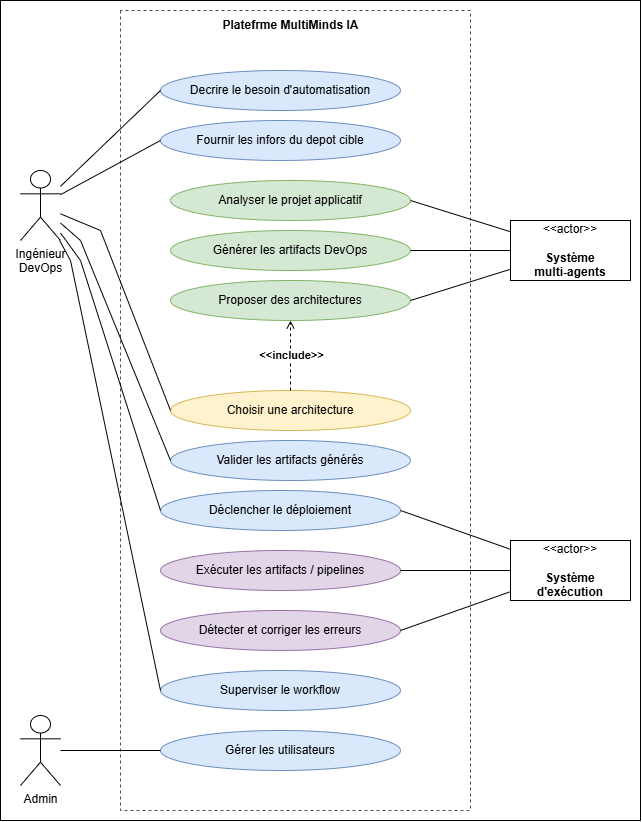
\includegraphics[width=0.85\textwidth]{images/Use_Case_Diagram.png}
    \caption{Diagramme global de cas d'utilisation de la plateforme}
    \label{fig:use-case-global}
\end{figure}

Le diagramme de la figure~\ref{fig:use-case-global} représente les principales
fonctionnalités de la plateforme et les acteurs concernés. L'ingénieur DevOps est l'acteur
déclencheur~: il décrit le besoin d'automatisation et fournit le dépôt cible. Le système
prend ensuite le relais à travers deux sous-systèmes représentés comme acteurs
secondaires~: le \textit{système multi-agents}, responsable de l'analyse du projet, de la
génération des artefacts DevOps et de la proposition d'architectures, et le \textit{système
d'exécution}, responsable de l'exécution des artefacts ainsi que de la détection et de la
correction des erreurs.

Cette représentation matérialise la frontière entre décision humaine et automatisation. Le
cas \textit{Choisir une architecture} est relié par une relation \texttt{<<include>>} au
cas \textit{Proposer des architectures}~: le choix suppose des propositions préalables. De
même, les cas \textit{Valider les artefacts générés} et \textit{Déclencher le déploiement}
placent l'utilisateur en position de contrôle avant toute action irréversible, ce qui
répond au besoin de validation humaine multi-étapes~; enfin, le cas \textit{Détecter et
corriger les erreurs}, porté par le système d'exécution, illustre la boucle de correction
détaillée plus loin.

\subsection{Vue structurelle}

\subsubsection{Diagramme d'activité}

\begin{figure}[htbp]
    \centering
    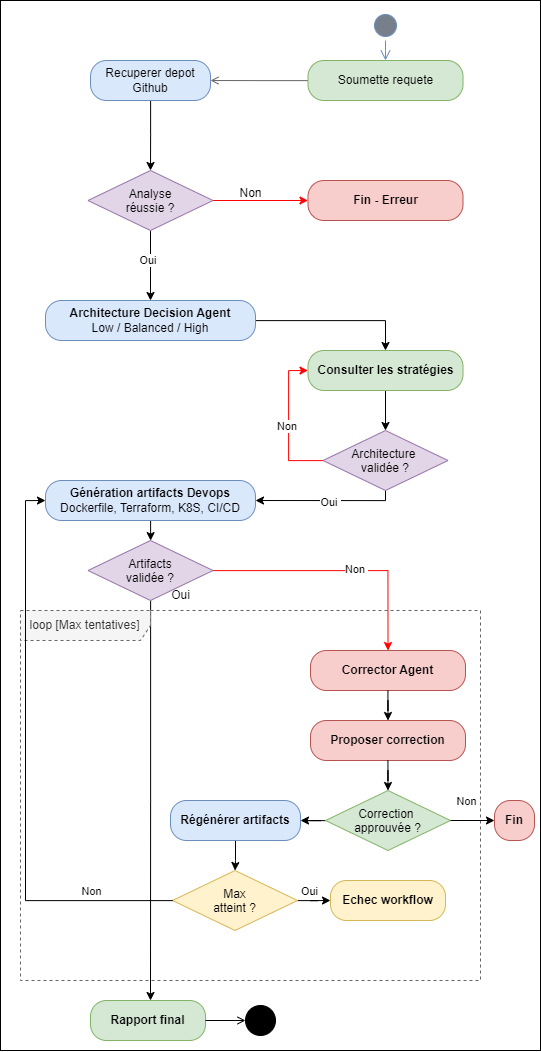
\includegraphics[width=0.62\textwidth]{images/Diag activité.png}
    \caption{Diagramme d'activité~--- déroulement global du workflow}
    \label{fig:activite-workflow}
\end{figure}

La figure~\ref{fig:activite-workflow} décrit l'organisation des traitements, de la
soumission de la requête jusqu'à la production du rapport final. Après récupération du
dépôt GitHub, une première condition vérifie le bon déroulement de l'analyse~; en cas
d'échec, le workflow se termine immédiatement.

Si l'analyse réussit, l'\textit{Architecture Decision Agent} propose plusieurs stratégies
(\textit{Low}, \textit{Balanced}, \textit{High}) que l'utilisateur valide ou non. Tant que
l'architecture n'est pas validée, le workflow revient à l'étape de consultation. Une fois
validée, le système génère les artefacts DevOps (Dockerfile, Terraform, Kubernetes, CI/CD),
à leur tour soumis à validation. En cas d'échec, le \textit{Corrector Agent} propose une
correction~: si elle est approuvée, les artefacts sont régénérés et revalidés, dans la
limite d'un nombre maximal de tentatives~; au-delà, le workflow échoue. Ce diagramme
synthétise ainsi les deux boucles de validation ---~architecture et artefacts~--- qui
structurent le pipeline.

\subsection{Vue dynamique}

\subsubsection{Diagramme de séquence}

\begin{figure}[htbp]
    \centering
    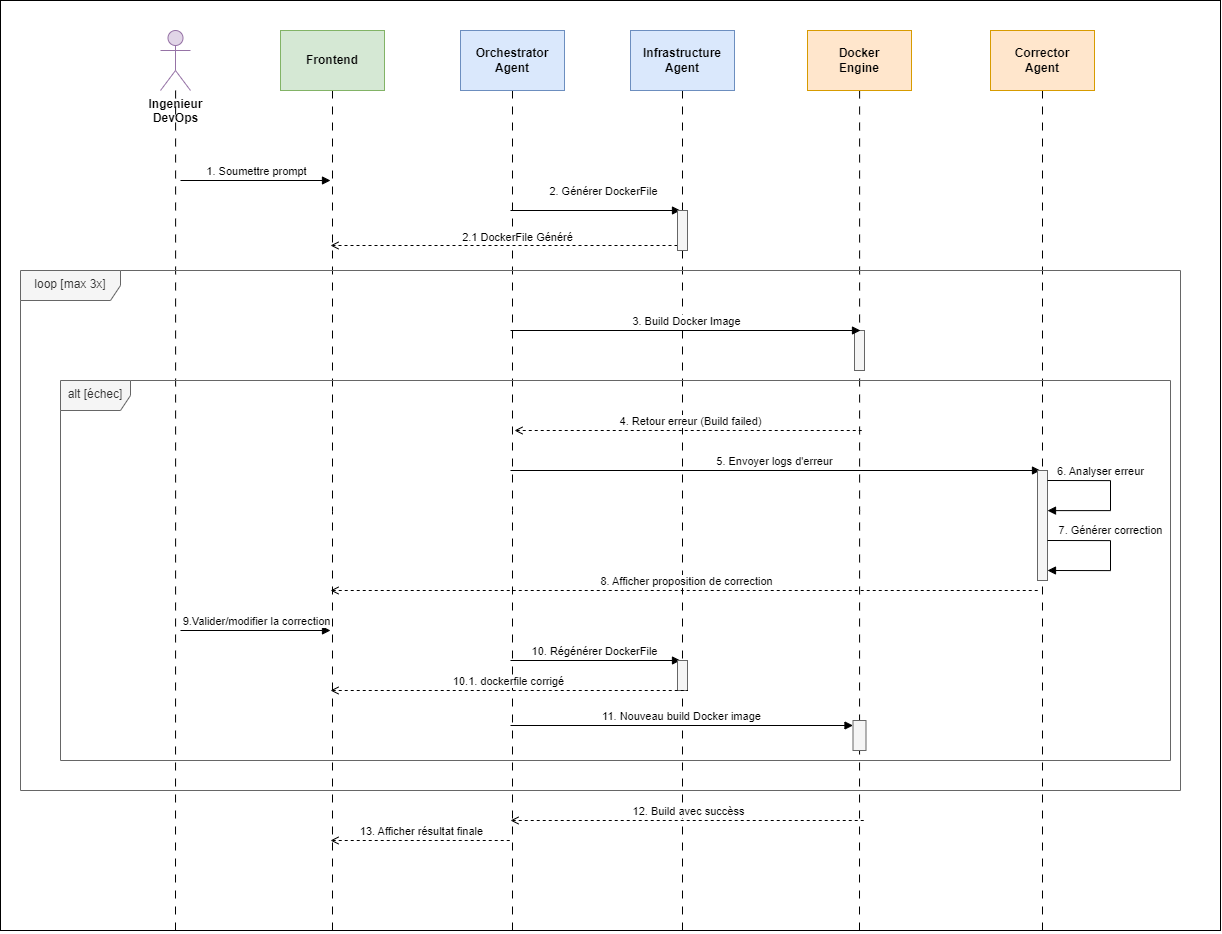
\includegraphics[width=0.90\textwidth]{images/Diag Sequence.png}
    \caption{Diagramme de séquence~--- génération et correction d'un Dockerfile}
    \label{fig:sequence-docker}
\end{figure}

La figure~\ref{fig:sequence-docker} illustre la génération d'un Dockerfile et sa correction
automatique en cas d'échec de build. L'ingénieur DevOps soumet un prompt via le frontend~;
celui-ci est transmis à l'\textit{Orchestrator Agent}, qui sollicite l'\textit{Infrastructure
Agent} pour générer le Dockerfile. Le fichier est ensuite construit par le \textit{Docker
Engine}, à l'intérieur d'une boucle bornée à trois tentatives.

Si le build échoue, l'erreur est remontée à l'orchestrateur, qui transmet les journaux au
\textit{Corrector Agent}. Ce dernier analyse l'erreur et génère une proposition de
correction, que l'ingénieur DevOps valide ou modifie avant régénération et nouveau build.
Lorsque le build aboutit, le résultat remonte à l'utilisateur. Ce scénario met en évidence
un point central de la conception~: la correction n'est jamais totalement automatique, elle
reste soumise à la validation de l'ingénieur, conformément au principe de validation humaine
multi-étapes.

\subsection{Architecture globale de la plateforme}

Les vues précédentes décrivent le système par facettes. La figure~\ref{fig:architecture-globale}
en donne une vision d'ensemble, du frontend jusqu'aux outils DevOps mobilisés le long du
pipeline.

\begin{figure}[htbp]
    \centering
    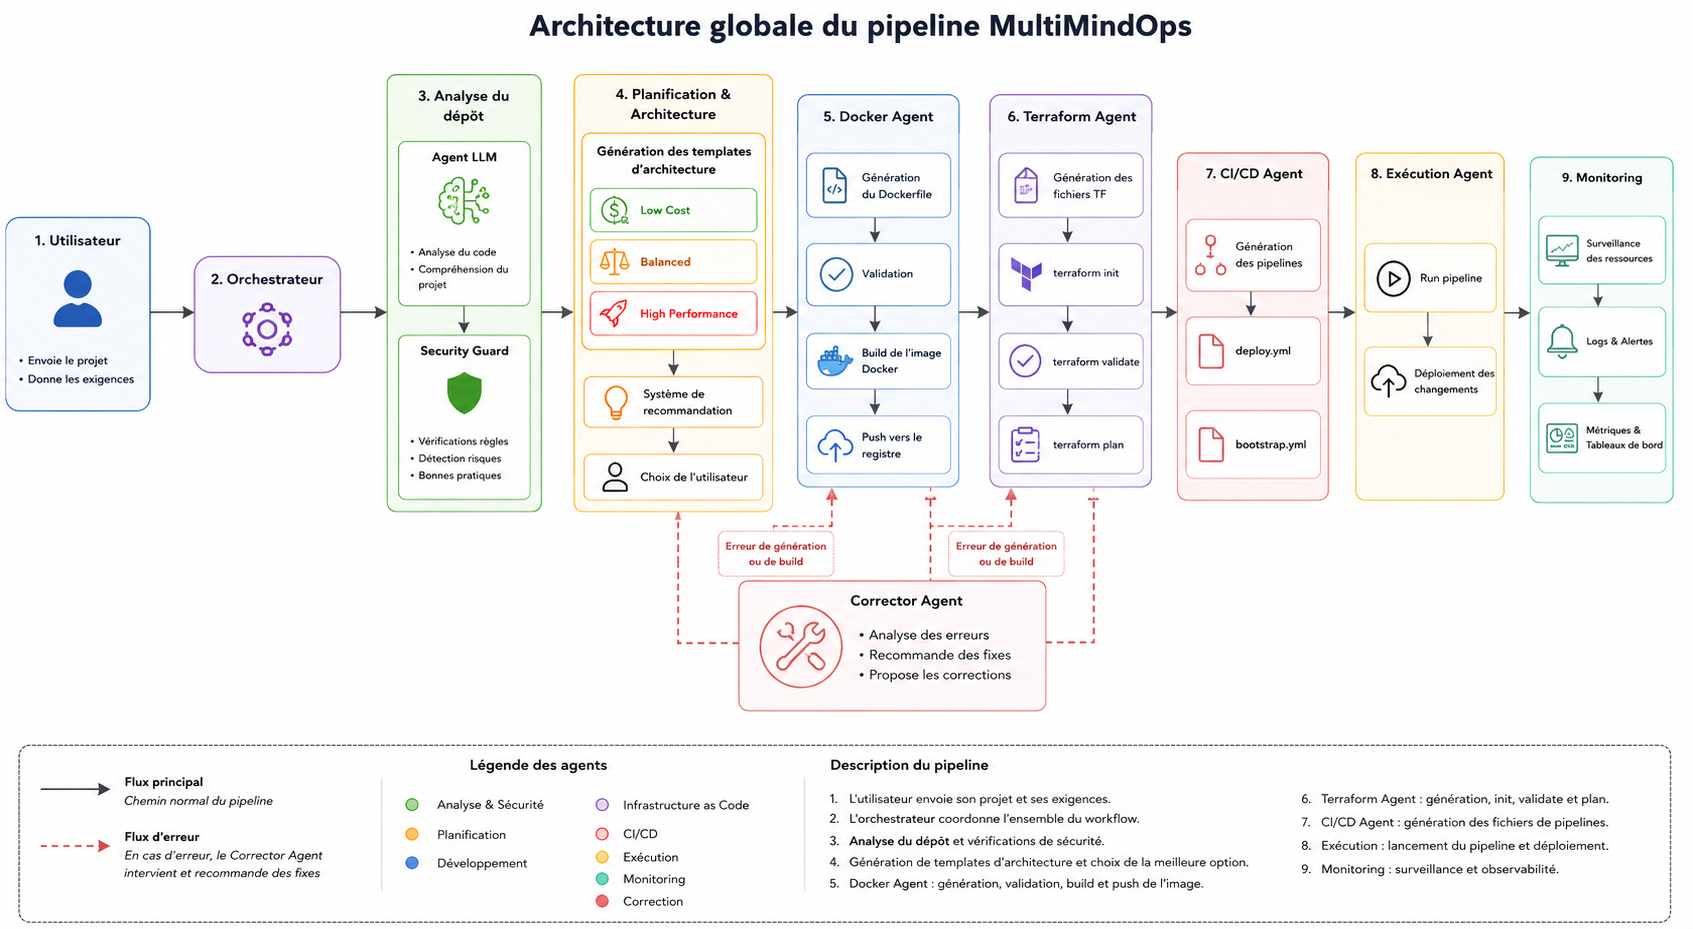
\includegraphics[width=\textwidth]{images/Diag architecture globale.png}
    \caption{Architecture globale de la plateforme MultiMindOps}
    \label{fig:architecture-globale}
\end{figure}

Le frontend communique avec le backend, qui orchestre les agents IA. Ces agents s'appuient
sur une base de connaissances RAG et sur des fournisseurs LLM pour raisonner, puis pilotent
les outils DevOps (Docker, Terraform, CI/CD) afin de produire et d'exécuter les artefacts.
Aux étapes critiques, une validation humaine intervient avant toute action, conformément au
principe \textit{Human-in-the-Loop}.

\section{Aperçu des capacités IA de MultiMindOps}

La valeur de la plateforme repose sur des agents IA spécialisés, chacun dédié à un type
d'artefact DevOps~: la remédiation intelligente des erreurs, la génération d'infrastructure
et la génération de pipelines CI/CD. Ces agents partagent un même socle technique
---~ancrage documentaire par RAG et fournisseur de raisonnement mutualisé~--- que nous
décrivons d'abord, avant de détailler les spécificités métier de chacun.

\subsection{Méthodologie d'évaluation et choix des modèles}

La comparaison qualitative des modèles ne repose pas sur une appréciation subjective, mais
sur la combinaison de plusieurs sources~: les benchmarks publics disponibles dans la
littérature, la documentation officielle des fournisseurs, les expérimentations menées dans
le cadre du projet, et une évaluation automatisée de la qualité des artefacts selon une
approche \textit{LLM-as-a-Judge}~\cite{LLM_AS_JUDGE}, où un modèle de langage note les
sorties d'après une grille prédéfinie. Le score final, exprimé sur~5, correspond à une
moyenne pondérée de plusieurs critères~: qualité des artefacts générés, cohérence
syntaxique, respect des bonnes pratiques, stabilité des réponses, temps de génération et
coût d'utilisation. Les valeurs rapportées dans ce chapitre découlent donc de cette
méthodologie, et non d'une estimation arbitraire.

\subsubsection{Fournisseur de raisonnement mutualisé}

Les trois agents reposent sur une architecture commune, ce qui permet de mutualiser le
choix du fournisseur principal. \textbf{GPT-5-mini} assure la compréhension du contexte, la
génération structurée et le raisonnement. \textbf{Llama~3.3~70B}, hébergé sur Groq,
n'intervient qu'en \textit{fallback} automatique~: il garantit la continuité du service en
cas d'indisponibilité ou de dépassement de quota du fournisseur principal. Ces deux modèles
occupant des rôles distincts~--- principal et secours~--- leur comparaison directe
apporterait peu~; l'analyse comparative est plutôt consacrée à un choix réellement
structurant pour la qualité des réponses~: le modèle d'\textit{embedding} du système RAG.

\subsubsection{Choix du modèle d'embedding pour le RAG}

La pertinence de la récupération documentaire dépend directement du modèle d'\textit{embedding}
retenu. Deux candidats ont été évalués selon la méthodologie précédente~:
\texttt{text-embedding-\allowbreak3-small} (OpenAI) et \texttt{nomic-embed-\allowbreak text-v1.5} (Nomic AI). La
qualité de recherche s'appuie sur les scores publiés du benchmark MTEB~\cite{MTEB}, les
autres critères provenant de la documentation des fournisseurs~\cite{OPENAI_DOCS,NOMIC_EMBED}
et des mesures réalisées dans le projet.

\begin{table}[htbp]
    \centering
    \caption{Comparaison des modèles d'\textit{embedding} candidats pour le système RAG}
    \label{tab:embedding-models}
    \footnotesize
    \begin{tabularx}{\textwidth}{@{}>{\raggedright\arraybackslash}p{3.4cm} c *{4}{>{\centering\arraybackslash}X} c@{}}
        \hline
        \textbf{Modèle} & \textbf{Dim.} & \textbf{Qualité de recherche} & \textbf{Coût} & \textbf{Temps d'encodage} & \textbf{Compat. RAG} & \textbf{Score (/5)} \\
        \hline
        \texttt{text-embedding-\allowbreak 3-small} & 1536 & $\approx$\,62 (MTEB) & API ($\approx$\,0,02\,\$/1\,M tok.) & Latence réseau & Native & \textbf{4,6} \\
        \texttt{nomic-embed-\allowbreak text-v1.5} & 768 & $\approx$\,62 (MTEB) & Gratuit (auto-hébergé) & Local, rapide & Bonne & 4,3 \\
        \hline
    \end{tabularx}
\end{table}

Les deux modèles offrent une qualité de recherche comparable sur MTEB. \texttt{text-embedding-\allowbreak3-small}
a néanmoins été retenu pour son intégration native à la pile OpenAI de la plateforme et sa
dimension supérieure (1536), au prix d'un coût d'API et d'une latence réseau que
\texttt{nomic-embed-\allowbreak text-v1.5} évite grâce à un hébergement local. Ce dernier demeure une
alternative crédible pour un déploiement entièrement auto-hébergé.

\subsection{Remédiation intelligente des erreurs (Corrector Agent)}

Le \textit{Corrector Agent} intervient lorsqu'un artefact échoue à une étape de build ou de
validation~: plutôt que d'interrompre le workflow, il diagnostique la cause de l'échec et
propose une correction ciblée, sous le contrôle de l'utilisateur.

\subsubsection{Architecture et workflow}

\begin{figure}[htbp]
    \centering
    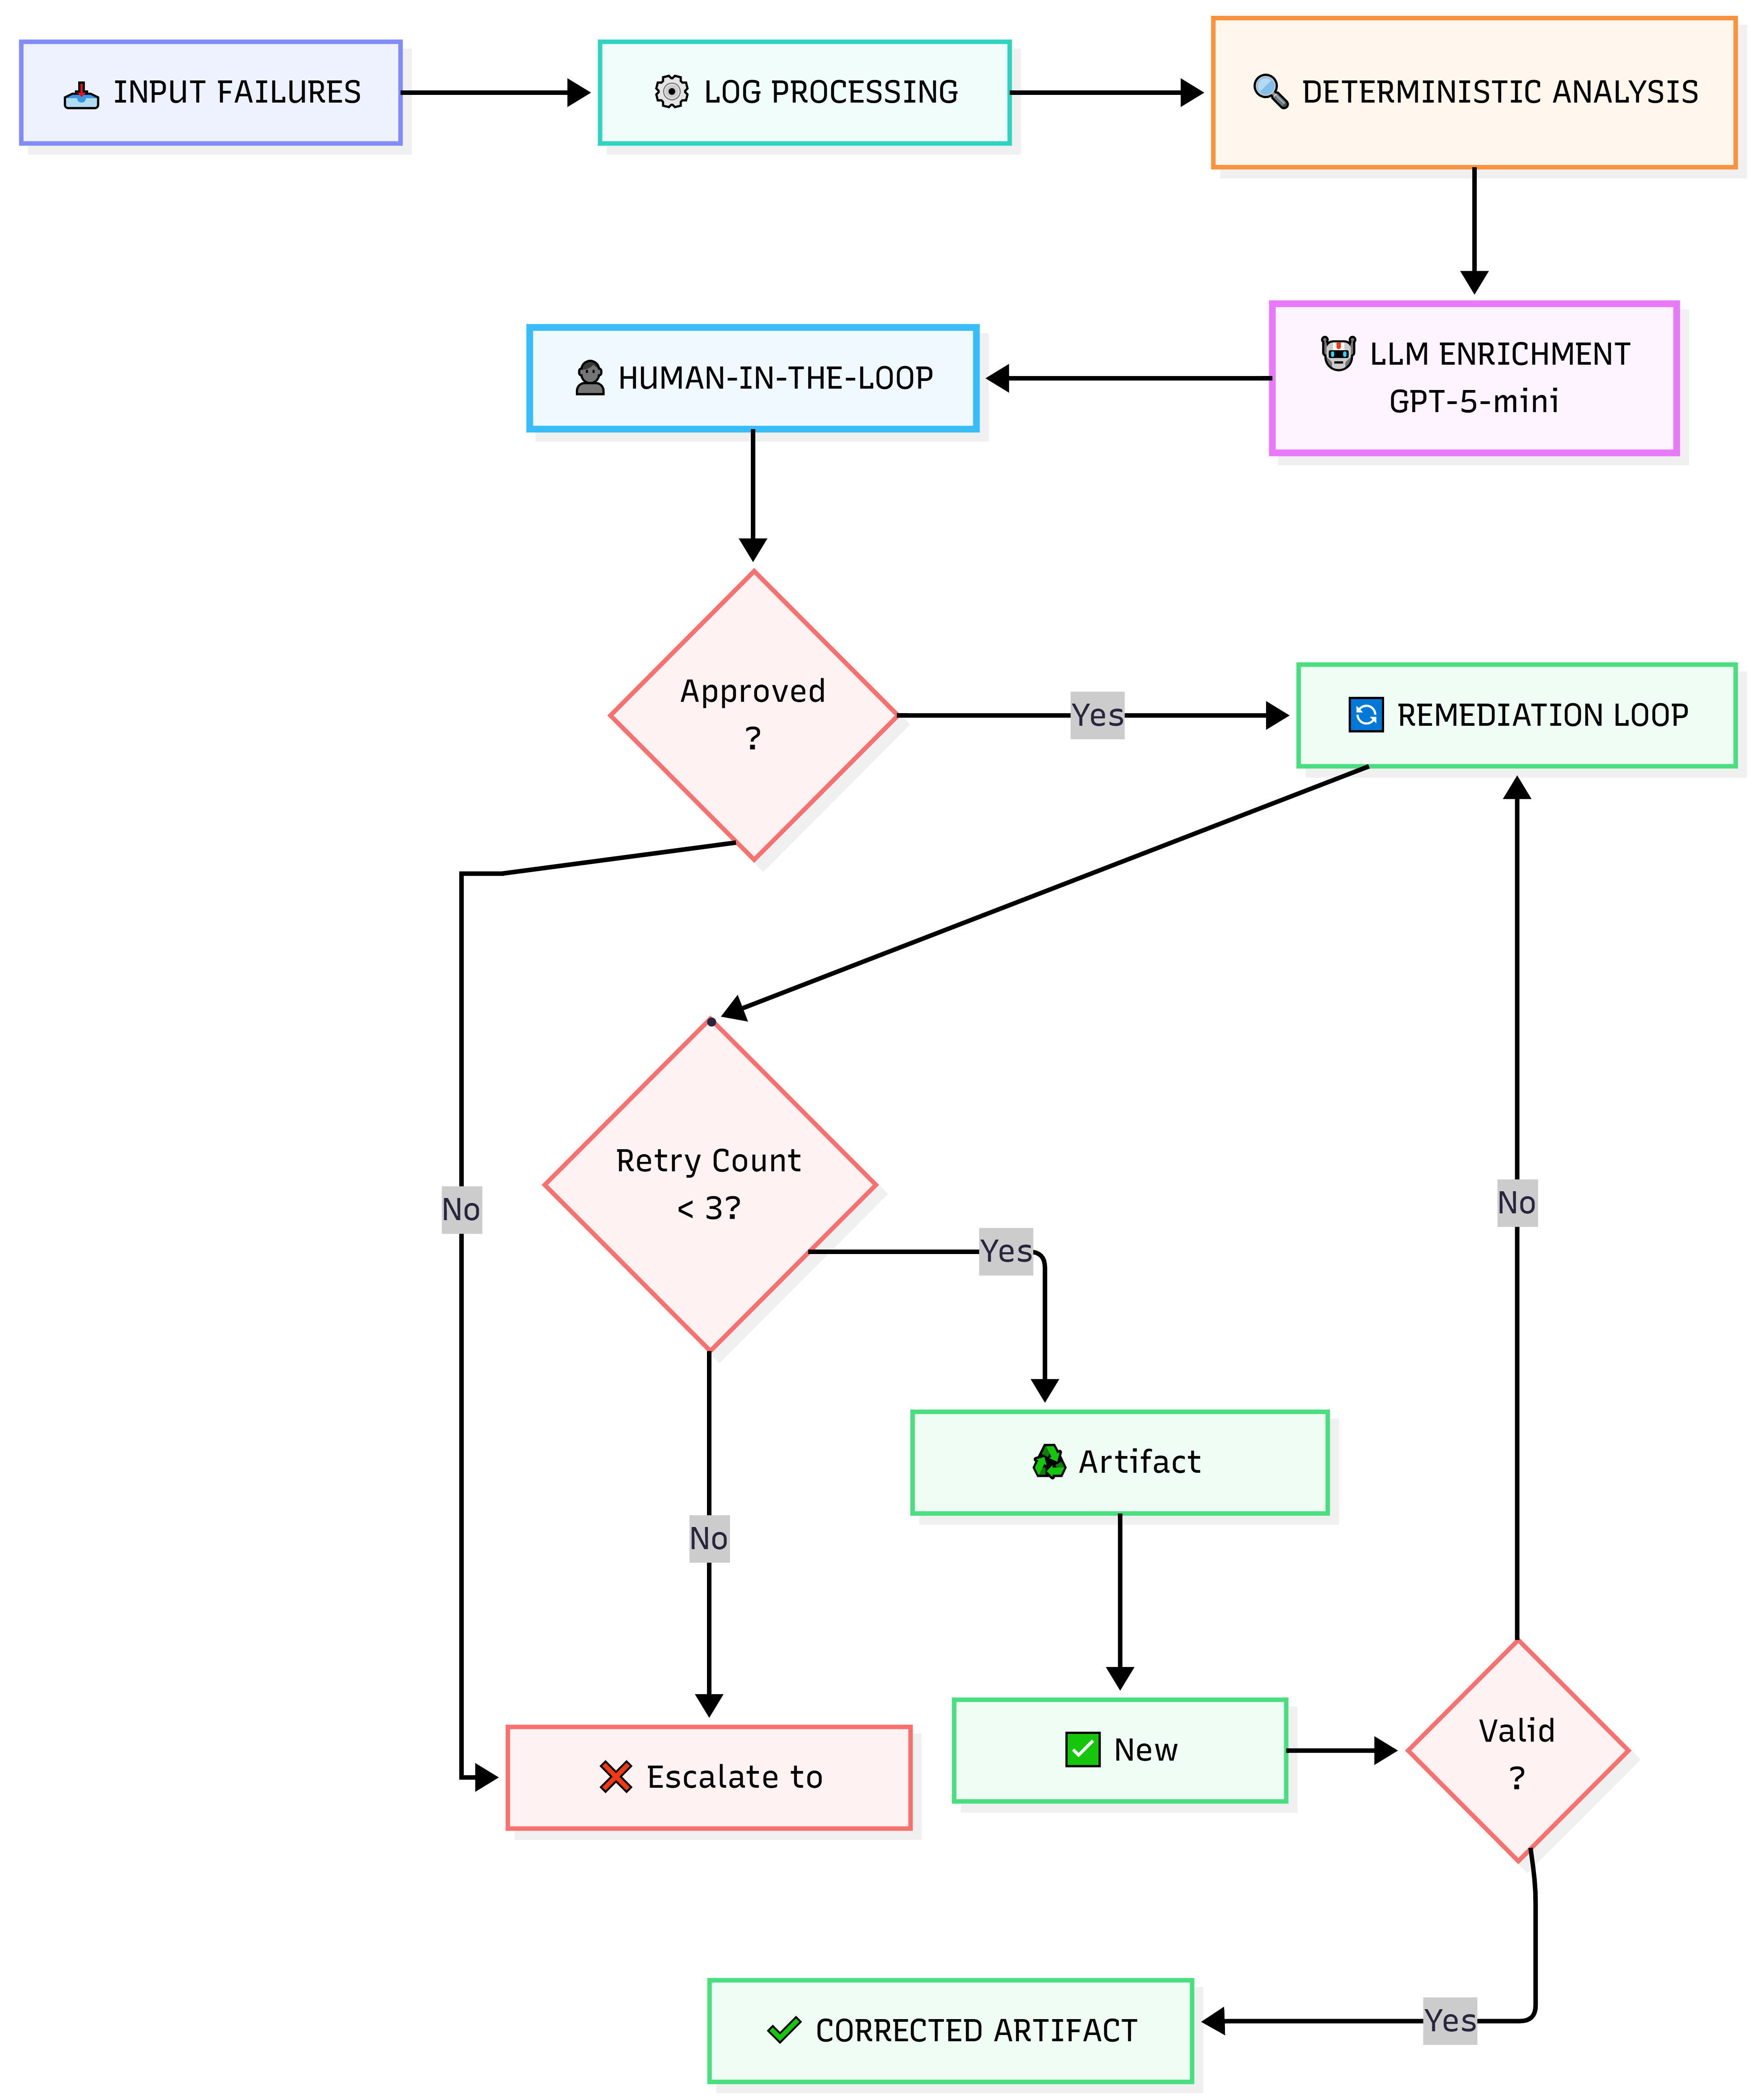
\includegraphics[width=0.85\textwidth]{images/Intelligent Error Remediation.png}
    \caption{Architecture fonctionnelle du \textit{Corrector Agent}}
    \label{fig:corrector-arch}
\end{figure}

Le workflow de la figure~\ref{fig:corrector-arch} repose sur un principe clé~: une analyse
déterministe précède le recours au modèle. Les journaux d'échec sont d'abord normalisés et
classifiés par des règles déterministes~; GPT-5-mini n'intervient qu'ensuite, pour enrichir
le diagnostic et formuler une correction. La proposition est soumise à l'utilisateur
(\textit{human-in-the-loop})~: une fois approuvée, elle alimente une boucle bornée à trois
tentatives qui régénère puis revalide l'artefact. En cas de succès, l'artefact corrigé est
livré~; sinon, ou si la limite est atteinte, le cas est escaladé. Ce séquencement
---~déterminisme d'abord, IA ensuite, validation humaine et boucle bornée~--- limite le
coût des appels au modèle et évite les corrections divergentes.

\begin{itemize}
    \item \textbf{Entrées :} les journaux d'une exécution en échec (build ou validation),
    l'artefact fautif et le contexte du projet associé.
    \item \textbf{Sorties :} un artefact corrigé et validé, ou une escalade documentée
    lorsque la boucle est épuisée, dans les deux cas tracée pour audit.
    \item \textbf{Base de connaissances (RAG) :} une base vectorisée des motifs d'erreurs
    récurrents et de leurs remédiations~; les passages pertinents sont injectés dans le
    contexte du modèle pour ancrer la correction sur des solutions éprouvées.
    \item \textbf{LLM utilisé :} GPT-5-mini, avec repli automatique sur Llama~3.3~70B.
\end{itemize}

\subsubsection{Justification métier}

La remédiation d'erreurs est la tâche la plus exigeante en \textbf{raisonnement} de la
plateforme~: l'agent doit interpréter des journaux hétérogènes, en inférer la cause profonde
et proposer une modification ciblée sans dégrader le reste de l'artefact. C'est cette
capacité d'analyse des logs et de raisonnement causal qui prime ici, et sur laquelle
GPT-5-mini se distingue des modèles légers, au diagnostic souvent superficiel. La régularité
de ses sorties limite en outre le nombre d'itérations de la boucle de correction, où chaque
tentative engage un appel au modèle.

\subsection{Génération d'infrastructure assistée par IA}

L'\textit{Infrastructure Agent} assure le provisionnement automatisé de l'infrastructure
cible~: à partir du contexte projet, il sélectionne une architecture adaptée et génère les
artefacts correspondants, prêts au déploiement.

\subsubsection{Architecture et workflow}

\begin{figure}[htbp]
    \centering
    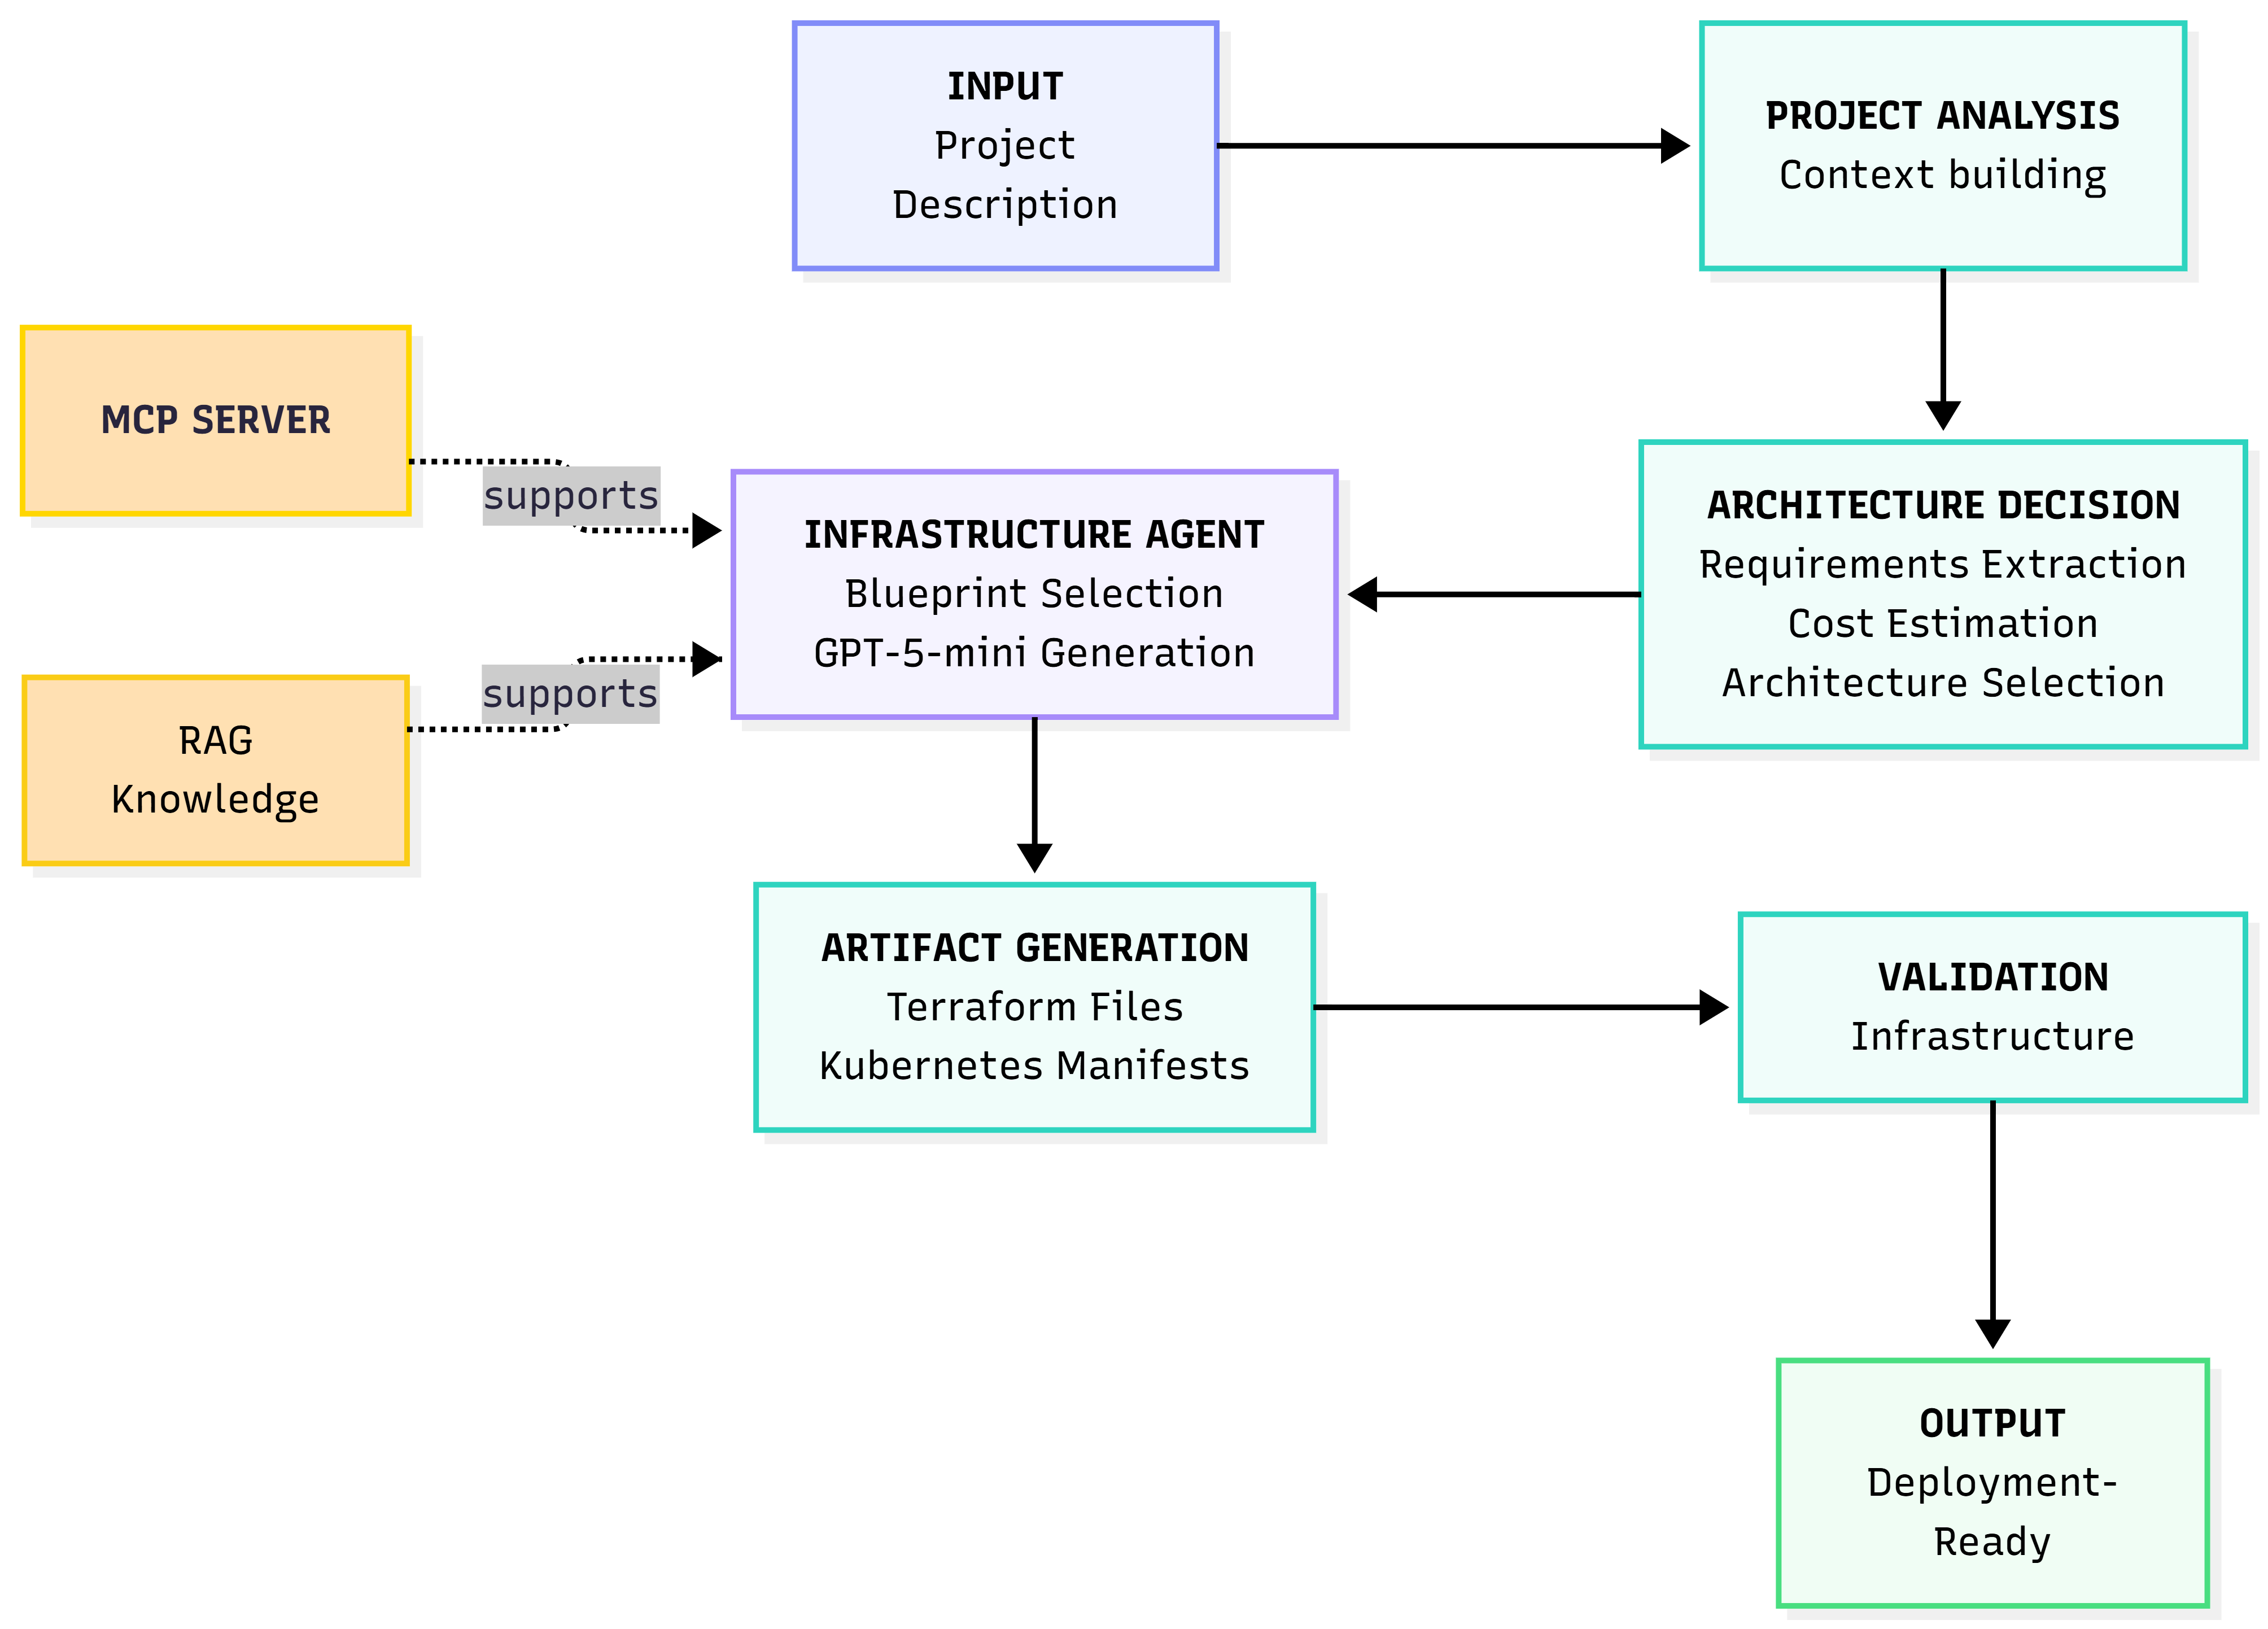
\includegraphics[width=0.90\textwidth]{images/Powered Infrastructure Generation.png}
    \caption{Architecture fonctionnelle de l'\textit{Infrastructure Agent}}
    \label{fig:infra-arch}
\end{figure}

Le workflow de la figure~\ref{fig:infra-arch} sépare trois responsabilités~: la décision,
la génération et la validation. Une phase d'analyse construit d'abord le contexte technique
du projet, puis une étape de décision combine extraction des besoins, estimation des coûts
et sélection de l'architecture la plus pertinente. L'\textit{Infrastructure Agent} exploite
cette décision pour choisir un \textit{blueprint} de référence et piloter la génération.
Deux services encadrent ce raisonnement~: le serveur MCP, qui fournit un accès outillé aux
ressources d'infrastructure, et la base RAG, qui ancre les sorties sur des références
éprouvées. Les artefacts produits sont enfin validés avant de constituer un livrable
déployable, ce qui garantit leur traçabilité et leur fiabilité.

\begin{itemize}
    \item \textbf{Entrées :} la description du projet et son contexte technique (besoins
    applicatifs, contraintes de déploiement, objectifs de coût).
    \item \textbf{Sorties :} des artefacts d'infrastructure validés et prêts au déploiement
    (fichiers Terraform et manifestes Kubernetes).
    \item \textbf{Base de connaissances (RAG) :} une base vectorisée des bonnes pratiques
    Terraform et Kubernetes, complétée par le serveur MCP qui expose les ressources
    d'infrastructure de façon structurée.
    \item \textbf{LLM utilisé :} GPT-5-mini, avec repli automatique sur Llama~3.3~70B.
\end{itemize}

\subsubsection{Justification métier}

La génération d'infrastructure exige des sorties longues, structurées et strictement
conformes à des schémas déclaratifs (HCL, YAML). L'enjeu central est ici le
\textbf{déterminisme}~: une configuration partiellement invalide échoue à la validation et
déclenche des reprises coûteuses. GPT-5-mini a été retenu pour sa capacité à produire des
artefacts valides dès la première passe, ce qui réduit les échecs de validation et fiabilise
l'estimation des coûts associée à l'architecture retenue.

\subsection{Génération de pipelines CI/CD assistée par IA}

Le \textit{CI/CD Agent} automatise la construction des pipelines d'intégration et de
déploiement continus~: à partir du contexte projet et de l'infrastructure définie, il génère
un pipeline complet et validé.

\subsubsection{Architecture et workflow}

\begin{figure}[htbp]
    \centering
    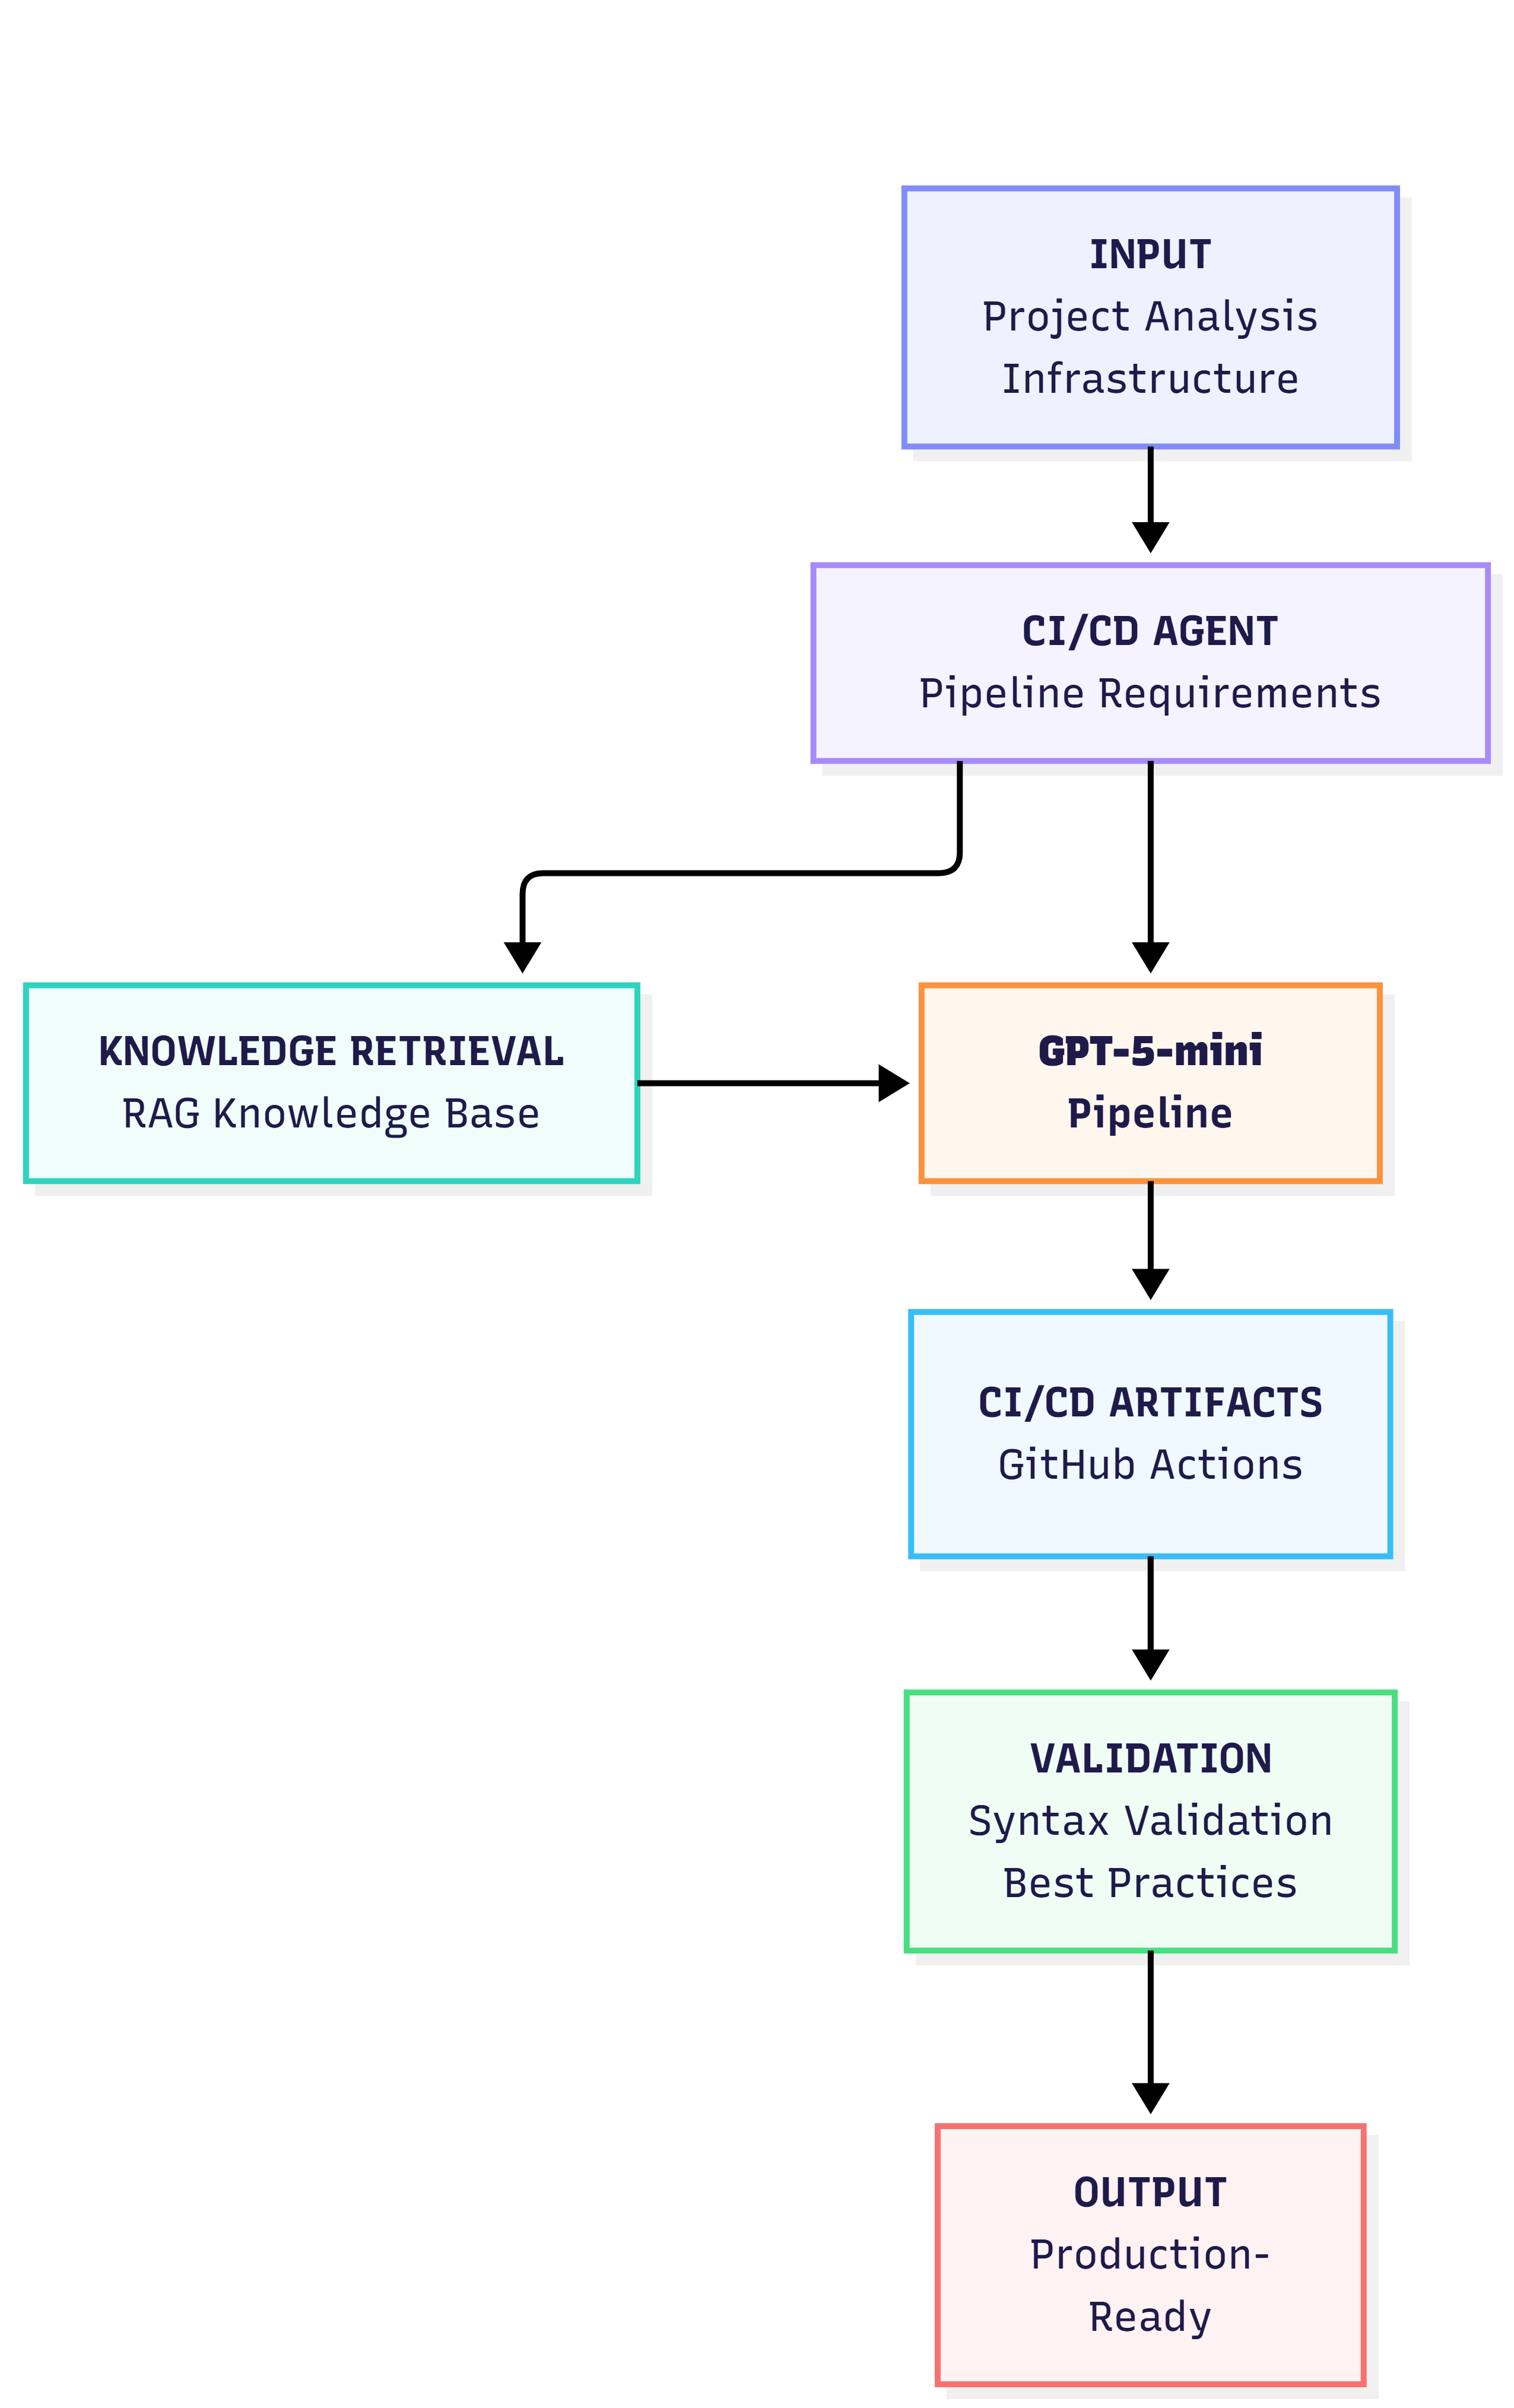
\includegraphics[width=0.72\textwidth]{images/AI-Powered CICD Generation.png}
    \caption{Architecture fonctionnelle du \textit{CI/CD Agent}}
    \label{fig:cicd-arch}
\end{figure}

Le workflow de la figure~\ref{fig:cicd-arch} part du contexte d'analyse du projet et de
l'infrastructure pour dériver les besoins du pipeline. Le \textit{CI/CD Agent} formalise ces
exigences, interroge la base RAG pour récupérer les références pertinentes (étapes de build,
conventions de déploiement) puis pilote la génération. Le pipeline est produit sous forme
d'artefacts CI/CD, avant une étape de validation portant sur la syntaxe et le respect des
bonnes pratiques. Les bonnes pratiques de sécurité sont intégrées directement aux artefacts
générés, comme propriété de qualité du pipeline plutôt que comme contrôle a posteriori.

\begin{itemize}
    \item \textbf{Entrées :} le contexte d'analyse du projet et les caractéristiques de
    l'infrastructure cible précédemment générée.
    \item \textbf{Sorties :} un pipeline CI/CD validé et prêt pour la production (workflows
    GitHub Actions).
    \item \textbf{Base de connaissances (RAG) :} une base vectorisée dédiée aux pratiques
    CI/CD~; les références adaptées sont injectées dans le raisonnement pour aligner les
    pipelines sur les standards de build et de déploiement.
    \item \textbf{LLM utilisé :} GPT-5-mini, avec repli automatique sur Llama~3.3~70B.
\end{itemize}

\subsubsection{Justification métier}

La génération de pipelines CI/CD repose sur la \textbf{cohérence des workflows YAML}~:
l'enchaînement des étapes (build, test, déploiement) doit être correct et les dépendances
entre \textit{jobs} respectées. Au-delà de la validité syntaxique, l'agent doit préserver la
logique globale du pipeline et y intégrer les bonnes pratiques comme propriété de qualité des
artefacts. GPT-5-mini assure cette cohérence de bout en bout avec une régularité supérieure
aux modèles évalués, tout en produisant des définitions YAML valides et maintenables.

\section{Conclusion}

Ce chapitre a formalisé les besoins de la plateforme, puis posé les bases de sa conception à
travers une modélisation UML couvrant les vues fonctionnelle, structurelle et dynamique, et
une architecture globale. Il a enfin détaillé les capacités d'intelligence artificielle qui
en constituent le c\oe ur, en explicitant l'architecture des agents spécialisés et une
méthodologie d'évaluation reposant sur des benchmarks publics, la documentation des
fournisseurs et une approche \textit{LLM-as-a-Judge}. Ces choix obéissent à une logique
commune~--- ancrage documentaire par RAG et fournisseur de raisonnement mutualisé
(GPT-5-mini, avec repli sur Llama~3.3~70B)~--- déclinée selon les exigences métier de chaque
agent. Le chapitre suivant présente la réalisation effective de la plateforme.

    \chapter{Réalisation et mise en œuvre}
\begin{spacing}{1.2}
\minitoc
\thispagestyle{MyStyle}
\end{spacing}
\clearpage

\section{Introduction}

Ce chapitre présente la concrétisation de la plateforme à partir de la conception
établie précédemment. Nous décrivons d'abord l'environnement de travail et les
technologies retenues, puis nous illustrons les principales interfaces homme-machine à
travers des captures d'écran commentées. Nous validons enfin les capacités
intelligentes du système ---~génération d'infrastructure, automatisation des pipelines
CI/CD et remédiation des erreurs~--- afin de démontrer le bon fonctionnement de la
solution réalisée.

\section{Environnement de développement}

La réalisation s'appuie sur un environnement combinant des outils de développement web
et un ensemble d'outils DevOps. Les sections suivantes en précisent les composantes
matérielles et logicielles.

\subsection{Environnement matériel}

Le développement a été mené sur un poste de travail dont les caractéristiques sont
résumées dans le tableau~\ref{tab:env-materiel}.

\begin{table}[H]
    \centering
    \caption{Environnement matériel}
    \label{tab:env-materiel}
    \begin{tabularx}{\textwidth}{@{}>{\raggedright\arraybackslash}p{5cm} >{\raggedright\arraybackslash}X@{}}
        \hline
        \textbf{Composant} & \textbf{Spécification} \\
        \hline
        Système d'exploitation & Windows 10 (64 bits) \\
        Mémoire vive (RAM) & 8 Go \\
        Carte graphique & Intel HD Graphics 620 \\
        \hline
    \end{tabularx}
\end{table}

\subsection{Environnement logiciel}

L'environnement logiciel regroupe les outils de développement web et les outils DevOps
mobilisés tout au long du projet (tableau~\ref{tab:env-logiciel}).

\begin{table}[H]
    \centering
    \caption{Environnement logiciel}
    \label{tab:env-logiciel}
    \begin{tabularx}{\textwidth}{@{}>{\raggedright\arraybackslash}p{4cm} >{\raggedright\arraybackslash}X@{}}
        \hline
        \textbf{Domaine} & \textbf{Technologies} \\
        \hline
        Développement web & Python 3.11, FastAPI, ReactJS, WebSocket, Swagger, Streamlit \\
        DevOps & Docker, AWS CLI, Git / GitHub, Terraform, Kubernetes \\
        \hline
    \end{tabularx}
\end{table}

\subsection{Technologies utilisées}

Les technologies retenues se répartissent en trois familles~: les technologies de
développement, les technologies DevOps et cloud, et les technologies d'intelligence
artificielle.

\subsubsection{Technologies de développement}

\begin{table}[H]
    \centering
    \caption{Technologies de développement}
    \label{tab:tech-dev}
    \begin{tabularx}{\textwidth}{@{}>{\raggedright\arraybackslash}p{3.2cm} >{\raggedright\arraybackslash}p{3.8cm} >{\raggedright\arraybackslash}X@{}}
        \hline
        \textbf{Technologie} & \textbf{Catégorie} & \textbf{Rôle} \\
        \hline
        Python 3.11 & Langage backend & Logique métier et agents \\
        FastAPI & Framework API & Exposition des services REST \\
        ReactJS & Framework frontend & Interface utilisateur \\
        WebSocket & Communication & Suivi temps réel des workflows \\
        Swagger & Documentation API & Description et test des endpoints \\
        Streamlit & Prototypage & Visualisation et démonstrations \\
        \hline
    \end{tabularx}
\end{table}

\subsubsection{Technologies DevOps et Cloud}

\begin{table}[H]
    \centering
    \caption{Technologies DevOps et cloud}
    \label{tab:tech-devops}
    \begin{tabularx}{\textwidth}{@{}>{\raggedright\arraybackslash}p{3.2cm} >{\raggedright\arraybackslash}p{3.8cm} >{\raggedright\arraybackslash}X@{}}
        \hline
        \textbf{Technologie} & \textbf{Catégorie} & \textbf{Rôle} \\
        \hline
        Docker & Conteneurisation & Build et exécution des images \\
        Terraform & Infrastructure as Code & Provisionnement de l'infrastructure \\
        Kubernetes & Orchestration & Déploiement des conteneurs \\
        AWS CLI & Cloud & Interaction avec les services AWS \\
        Git / GitHub & Gestion de versions & Suivi du code et hébergement des dépôts \\
        \hline
    \end{tabularx}
\end{table}

\subsubsection{Technologies IA et Agents intelligents}

\begin{table}[H]
    \centering
    \caption{Technologies IA et agents intelligents}
    \label{tab:tech-ia}
    \begin{tabularx}{\textwidth}{@{}>{\raggedright\arraybackslash}p{3.2cm} >{\raggedright\arraybackslash}p{3.8cm} >{\raggedright\arraybackslash}X@{}}
        \hline
        \textbf{Technologie} & \textbf{Catégorie} & \textbf{Rôle} \\
        \hline
        LangGraph & Orchestration d'agents & Graphes d'états des workflows multi-agents \\
        LangChain & Framework LLM & Chaînage des appels et des outils \\
        Qdrant & Base vectorielle & Stockage et recherche RAG \\
        Groq API & Fournisseur LLM & Inférence de repli (\textit{fallback}) \\
        Lightning AI & Plateforme IA & Environnement de calcul et d'exécution \\
        OpenAI & Fournisseur LLM & Modèle de raisonnement principal (GPT-5-mini) \\
        MCP & Protocole d'outils & Accès outillé aux ressources d'infrastructure \\
        \hline
    \end{tabularx}
\end{table}

\section{Interfaces Homme-Machine}

Cette section présente les principales interfaces de la plateforme. Chaque capture est
accompagnée d'une brève description mettant en évidence la fonctionnalité illustrée.

\subsection{Authentification et gestion des utilisateurs}

La plateforme propose un accès sécurisé ainsi qu'une gestion des membres au sein d'un
espace de travail collaboratif.

\begin{figure}[H]
    \centering
    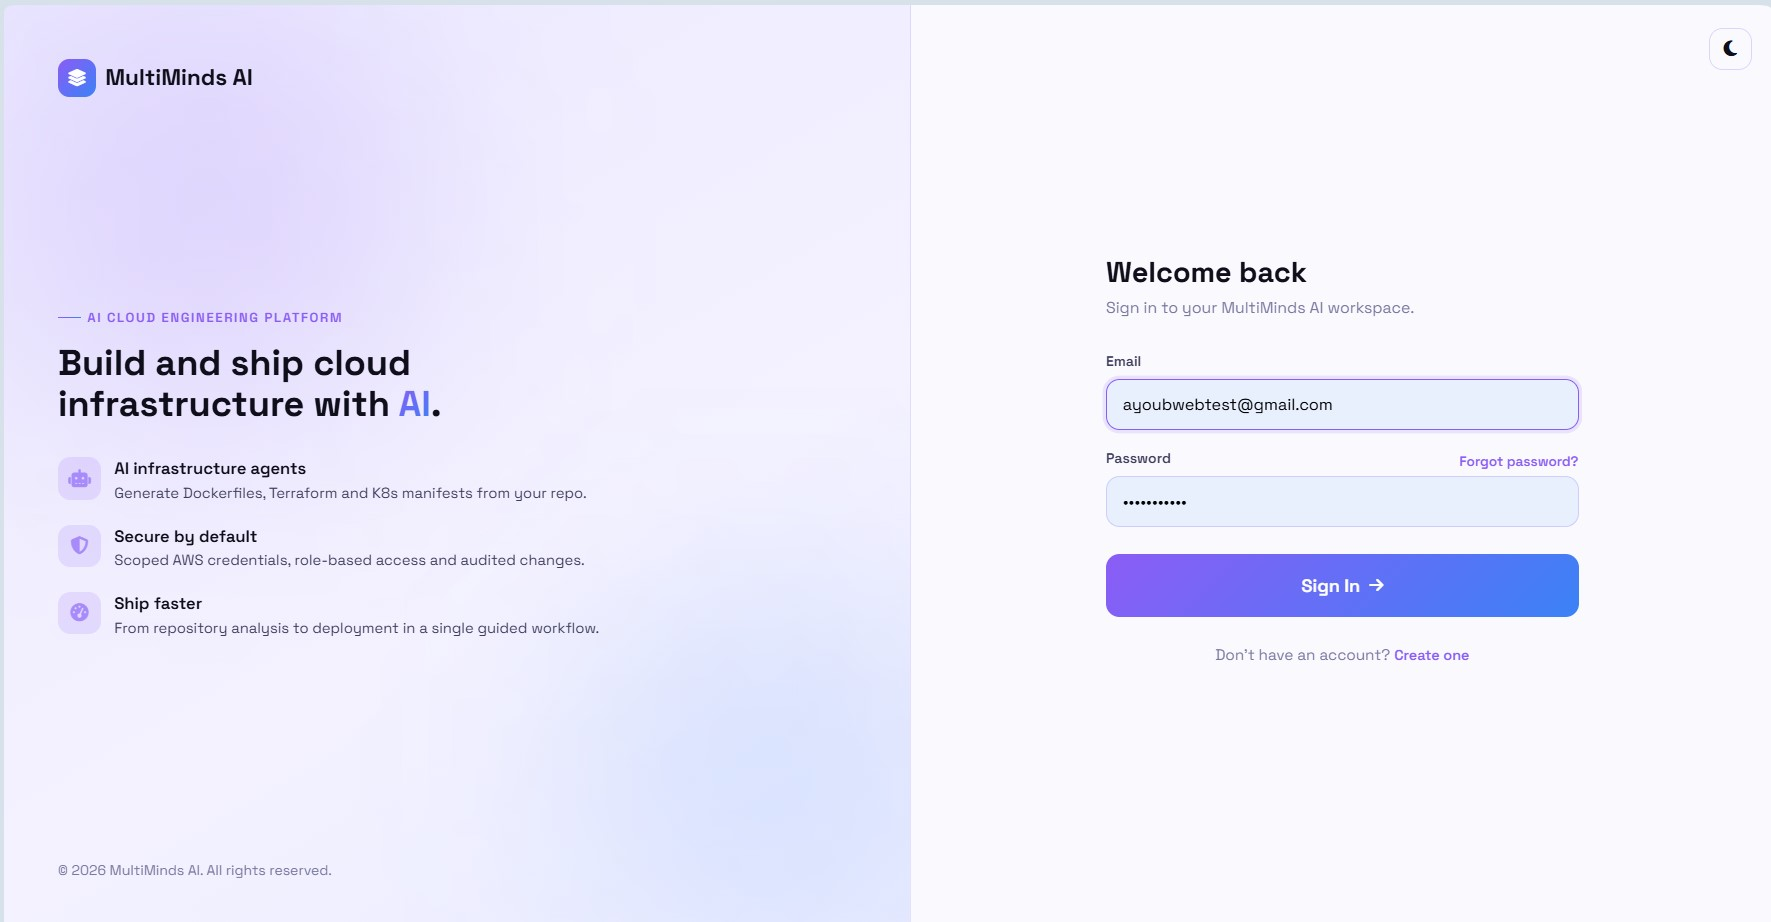
\includegraphics[width=0.75\textwidth]{images/Sign_in_page.jpg}
    \caption{Page d'authentification}
    \label{fig:sign-in}
\end{figure}

La figure~\ref{fig:sign-in} présente l'interface de connexion. L'utilisateur s'authentifie
à l'aide de ses identifiants pour accéder à son espace de travail et à ses projets.

\begin{figure}[H]
    \centering
    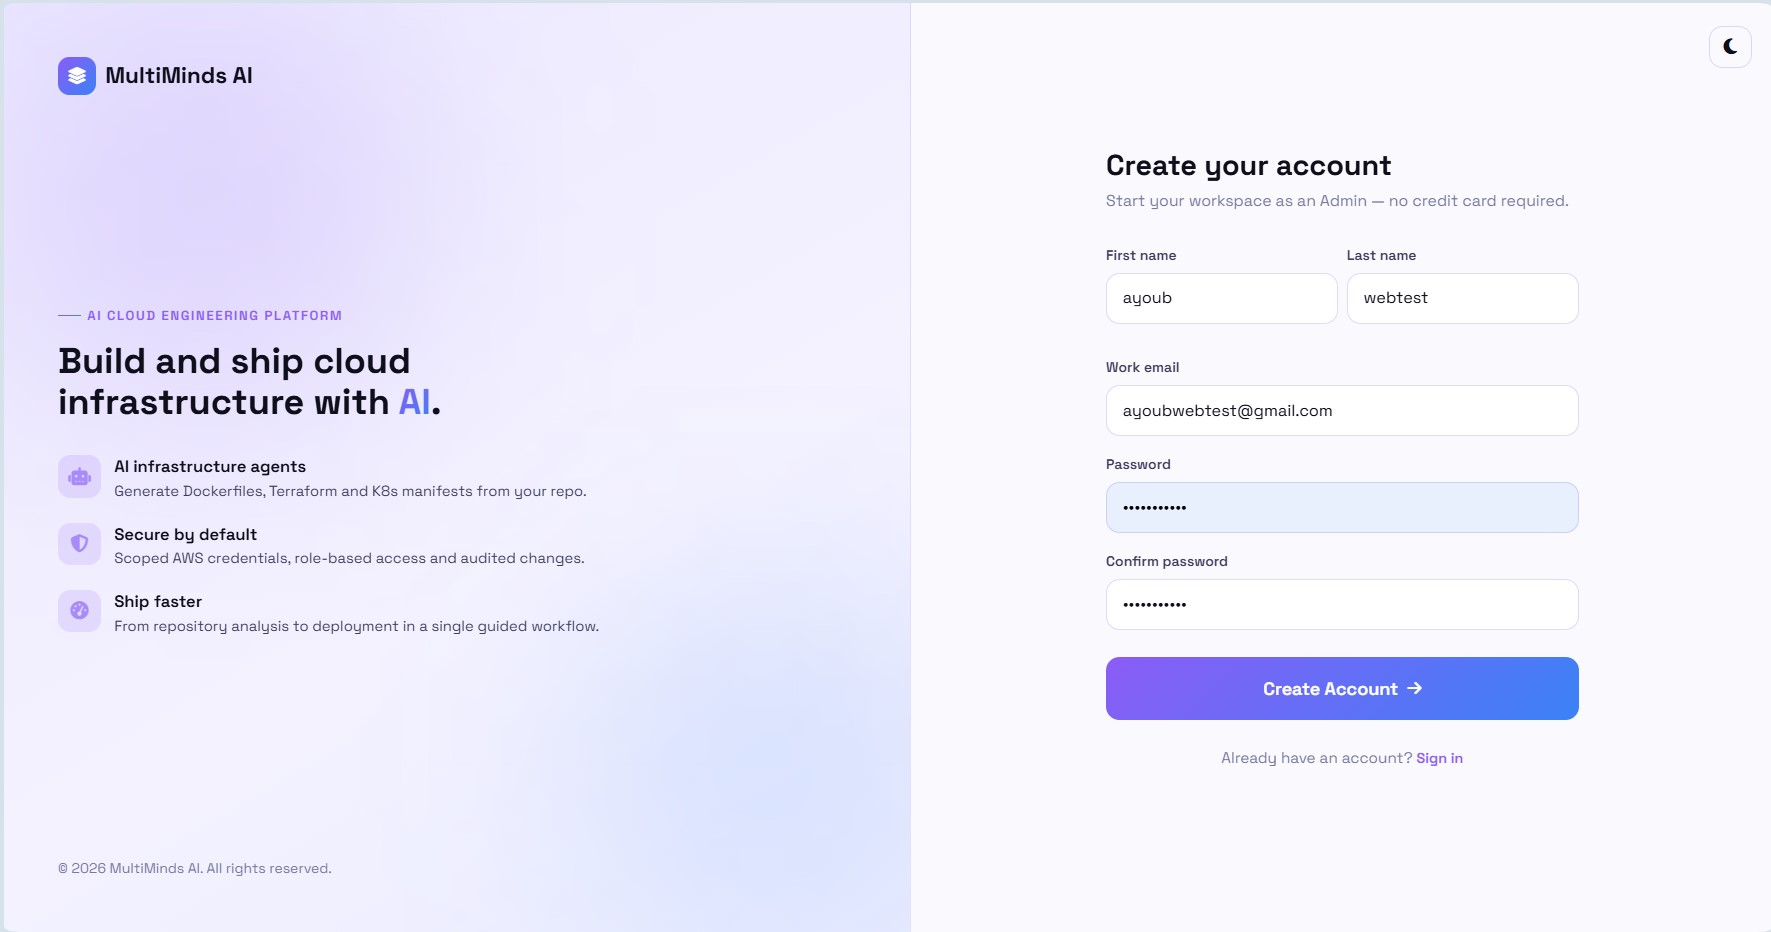
\includegraphics[width=0.75\textwidth]{images/Sign_up_page.jpg}
    \caption{Page d'inscription}
    \label{fig:sign-up}
\end{figure}

La figure~\ref{fig:sign-up} montre le formulaire de création de compte. Il permet à un
nouvel utilisateur de s'enregistrer avant de rejoindre ou de créer un espace de travail.

\begin{figure}[H]
    \centering
    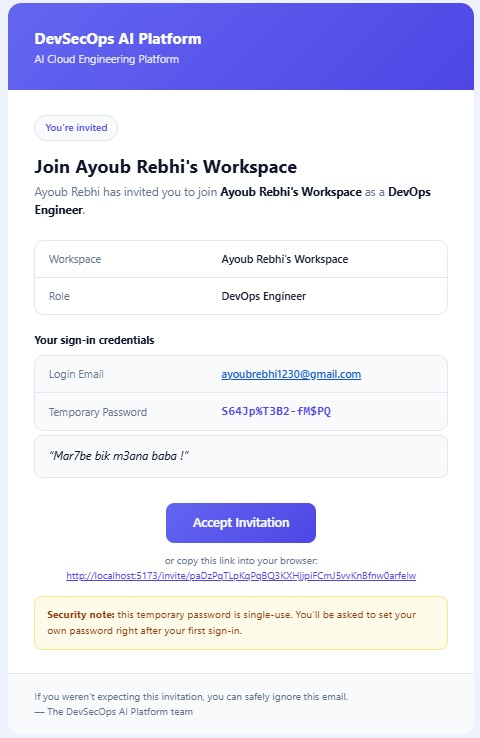
\includegraphics[width=0.75\textwidth]{images/invitation_mail.jpg}
    \caption{Courriel d'invitation}
    \label{fig:invitation-mail}
\end{figure}

La figure~\ref{fig:invitation-mail} illustre le courriel d'invitation envoyé
automatiquement à un membre. Il contient les informations d'accès nécessaires pour
rejoindre l'espace de travail.

\begin{figure}[H]
    \centering
    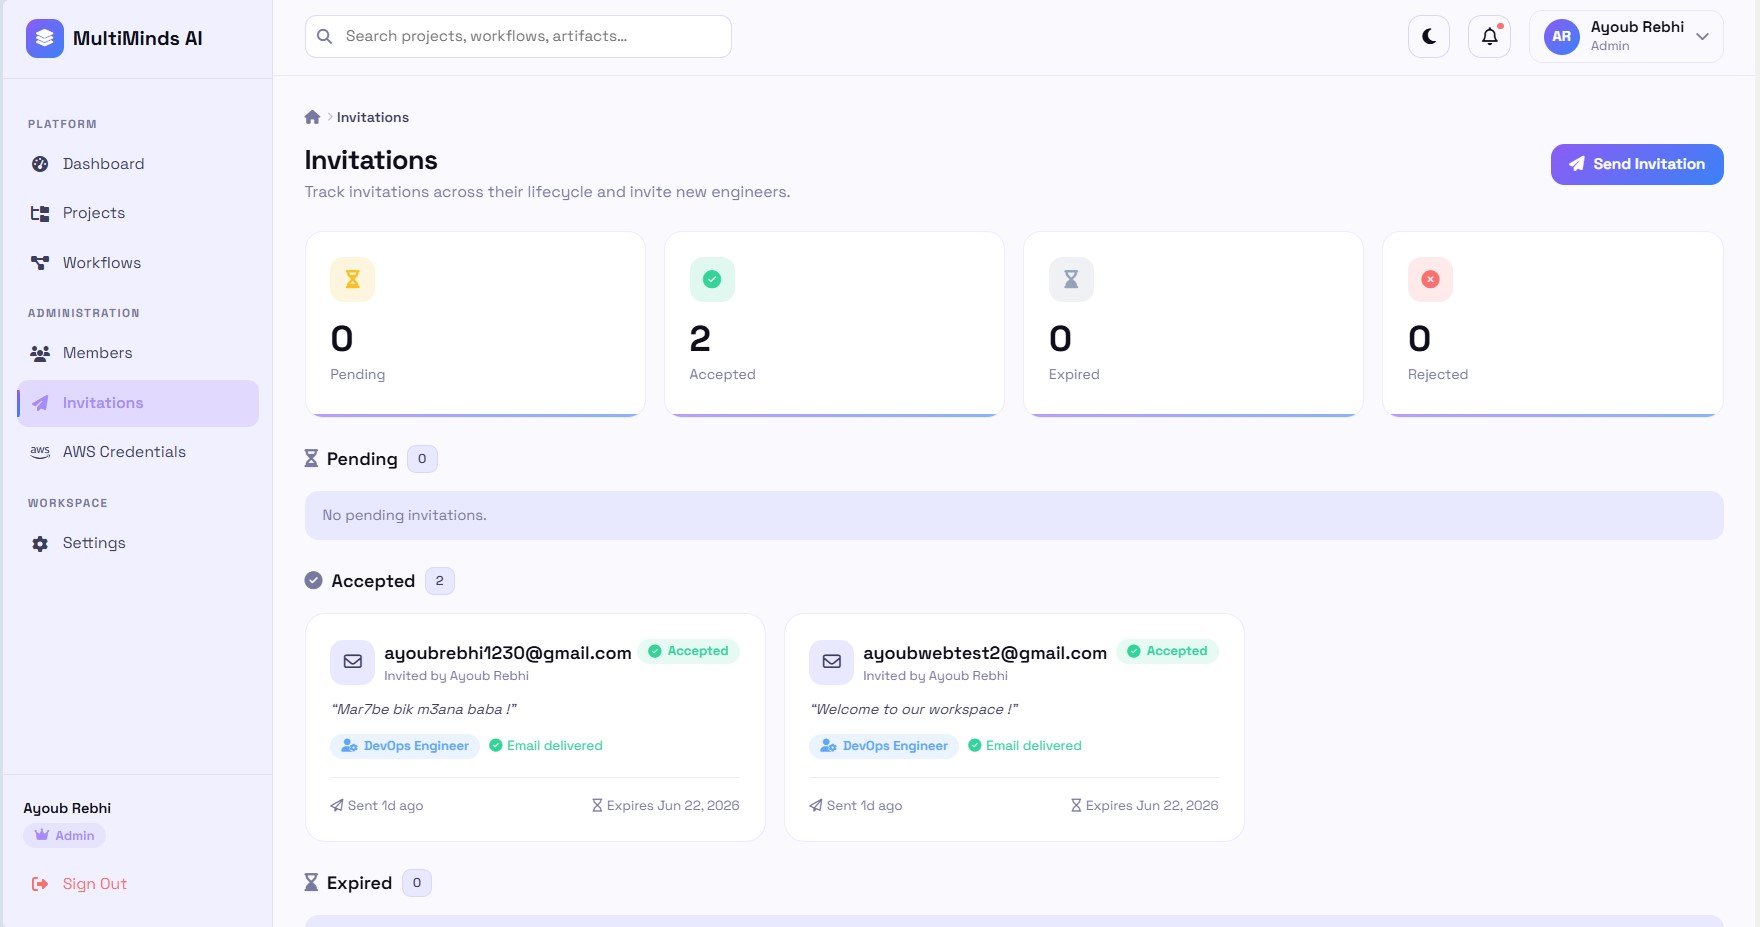
\includegraphics[width=0.85\textwidth]{images/Invite_members_to_workspace.jpg}
    \caption{Invitation de membres à l'espace de travail}
    \label{fig:invite-members}
\end{figure}

La figure~\ref{fig:invite-members} présente l'interface d'invitation des membres.
L'administrateur y ajoute de nouveaux collaborateurs et leur attribue un rôle.

\subsection{Tableau de bord et gestion des projets}

Le tableau de bord offre une vue d'ensemble de l'activité et donne accès à l'analyse
détaillée de chaque projet.

\begin{figure}[H]
    \centering
    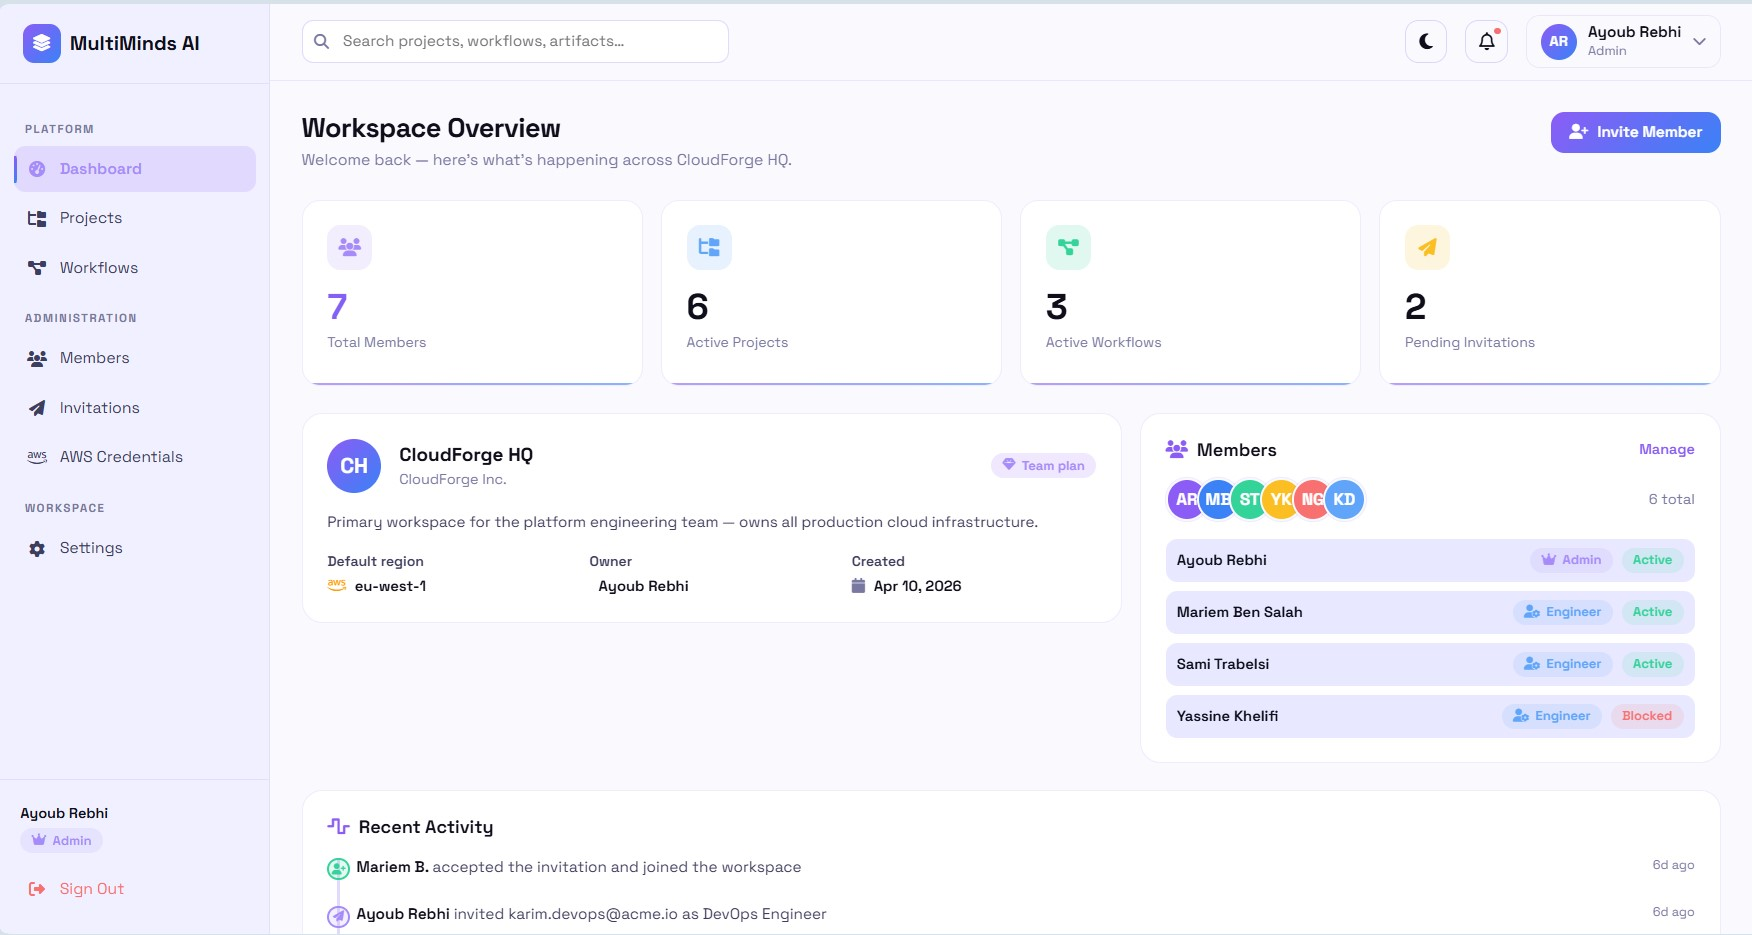
\includegraphics[width=0.9\textwidth]{images/Dashboard_admin.jpg}
    \caption{Tableau de bord administrateur}
    \label{fig:dashboard-admin}
\end{figure}

La figure~\ref{fig:dashboard-admin} présente le tableau de bord de l'administrateur. Il
synthétise l'état des projets, des workflows et des ressources gérées par la plateforme.

\begin{figure}[H]
    \centering
    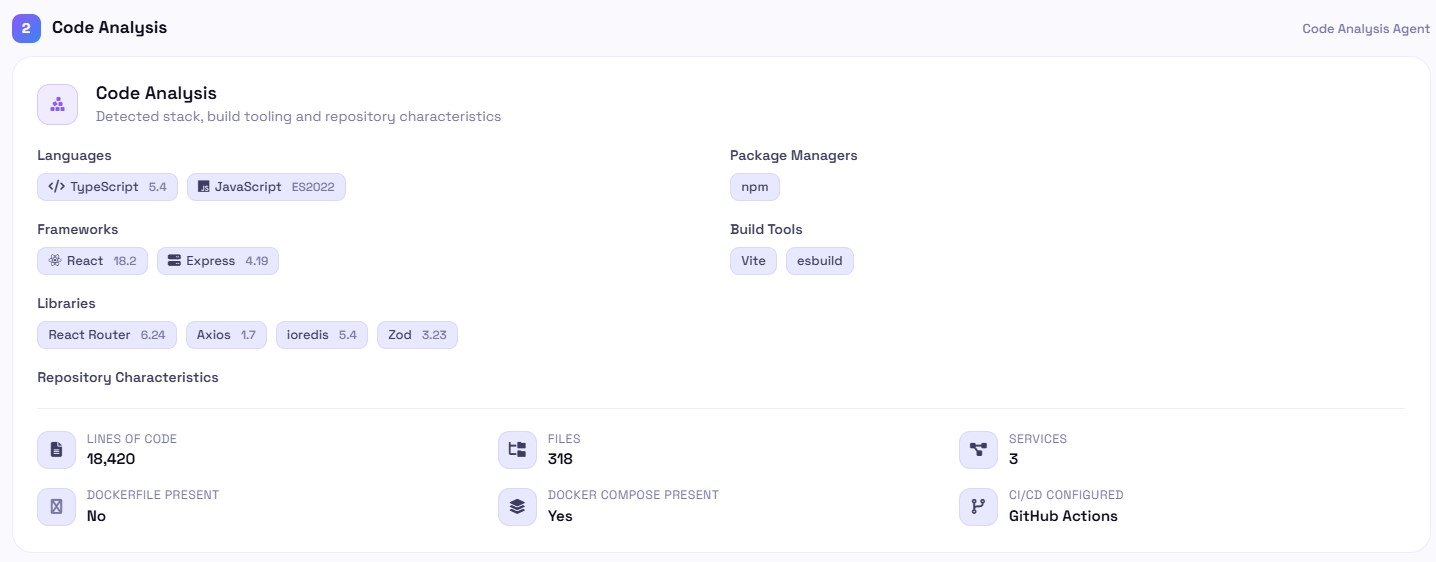
\includegraphics[width=0.9\textwidth]{images/Project_Analysis.jpg}
    \caption{Analyse d'un projet}
    \label{fig:project-analysis}
\end{figure}

La figure~\ref{fig:project-analysis} montre le résultat de l'analyse automatique d'un
projet. La plateforme identifie le langage, le framework et les dépendances afin de
guider les étapes suivantes du workflow.

\subsection{Sélection des architectures cloud}

À partir de l'analyse du projet, la plateforme propose plusieurs stratégies
d'architecture parmi lesquelles l'utilisateur effectue son choix.

\begin{figure}[H]
    \centering
    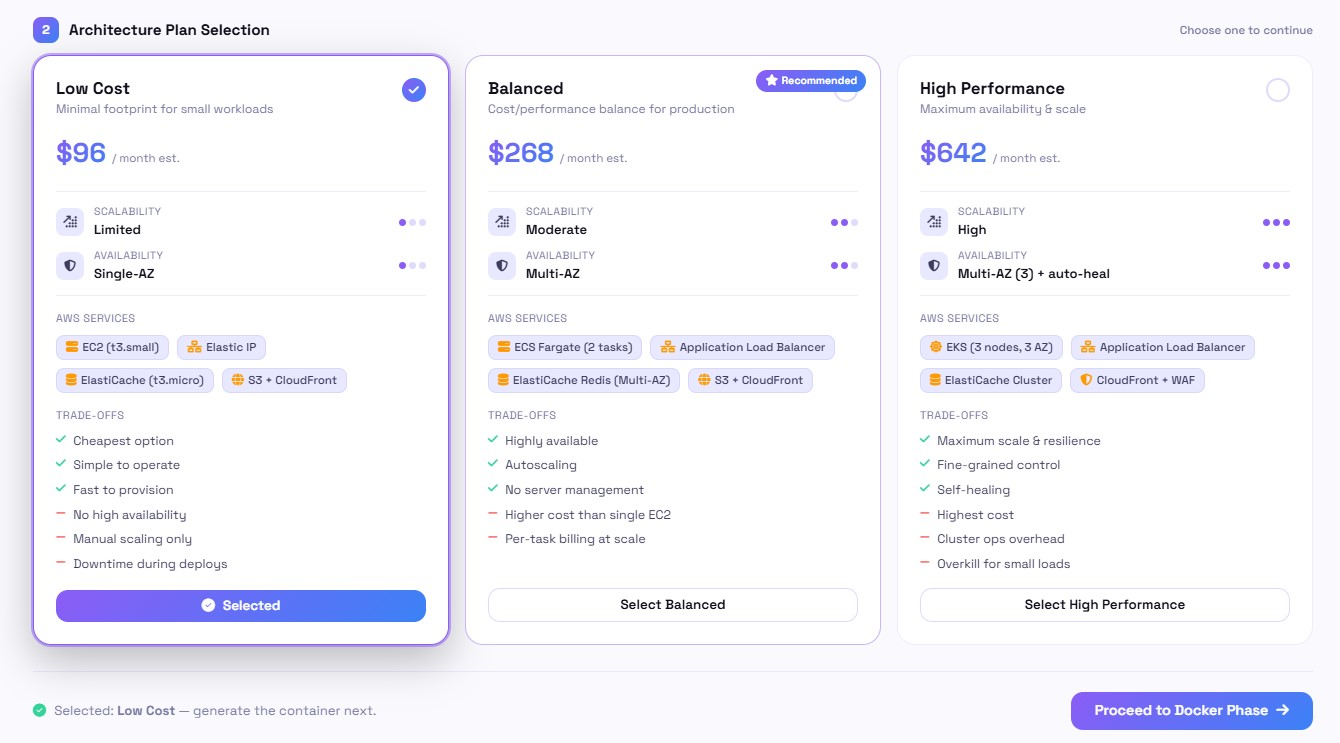
\includegraphics[width=0.9\textwidth]{images/Architecture plan selection.jpg}
    \caption{Sélection d'une architecture cloud}
    \label{fig:architecture-selection}
\end{figure}

La figure~\ref{fig:architecture-selection} présente les stratégies d'architecture
proposées (par exemple \textit{Low Cost}, \textit{Balanced}, \textit{High Performance}),
accompagnées d'une estimation de coût. L'utilisateur sélectionne l'option la mieux
adaptée à ses contraintes.

\subsection{Génération intelligente des artefacts DevOps}

La plateforme génère automatiquement les artefacts nécessaires au déploiement~:
Dockerfile, fichiers Terraform et pipelines CI/CD.

\begin{figure}[H]
    \centering
    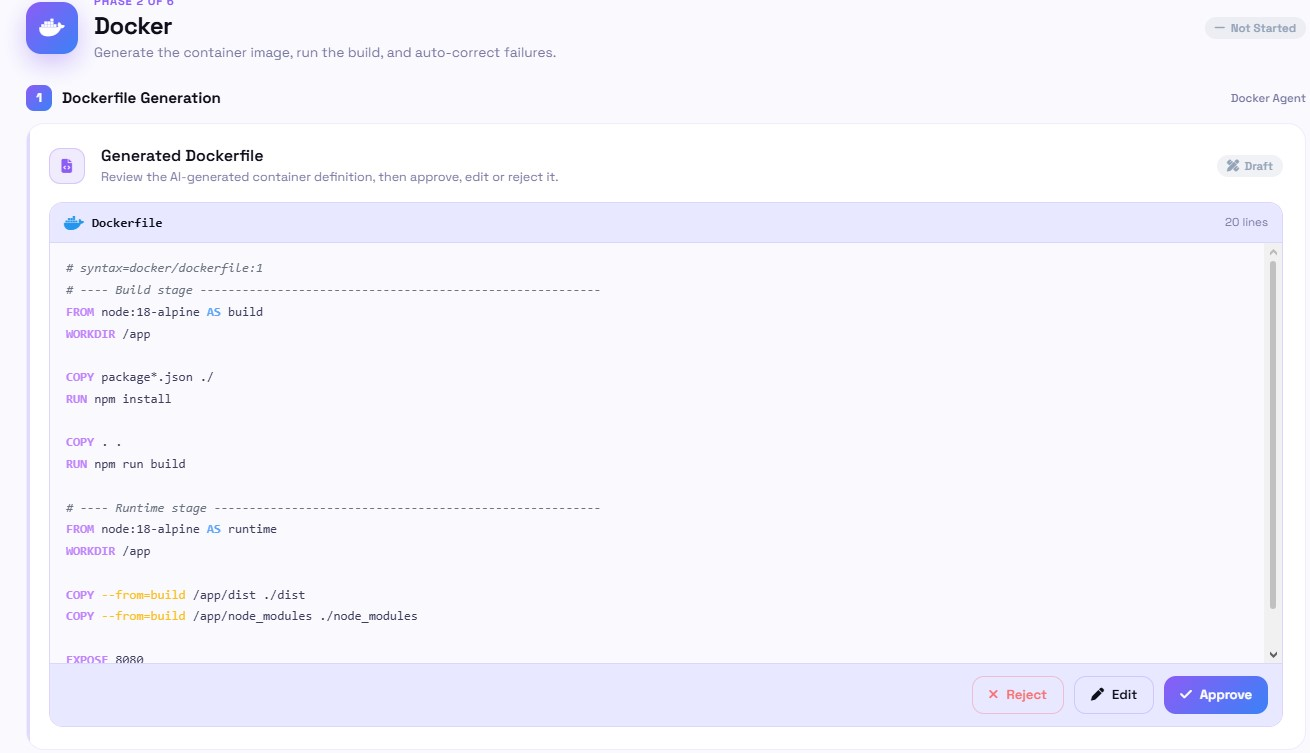
\includegraphics[width=0.9\textwidth]{images/Docker generation.jpg}
    \caption{Génération du Dockerfile}
    \label{fig:docker-generation}
\end{figure}

La figure~\ref{fig:docker-generation} illustre la génération d'un Dockerfile adapté au
projet, tenant compte du langage et des bonnes pratiques de sécurité et d'optimisation.

\begin{figure}[H]
    \centering
    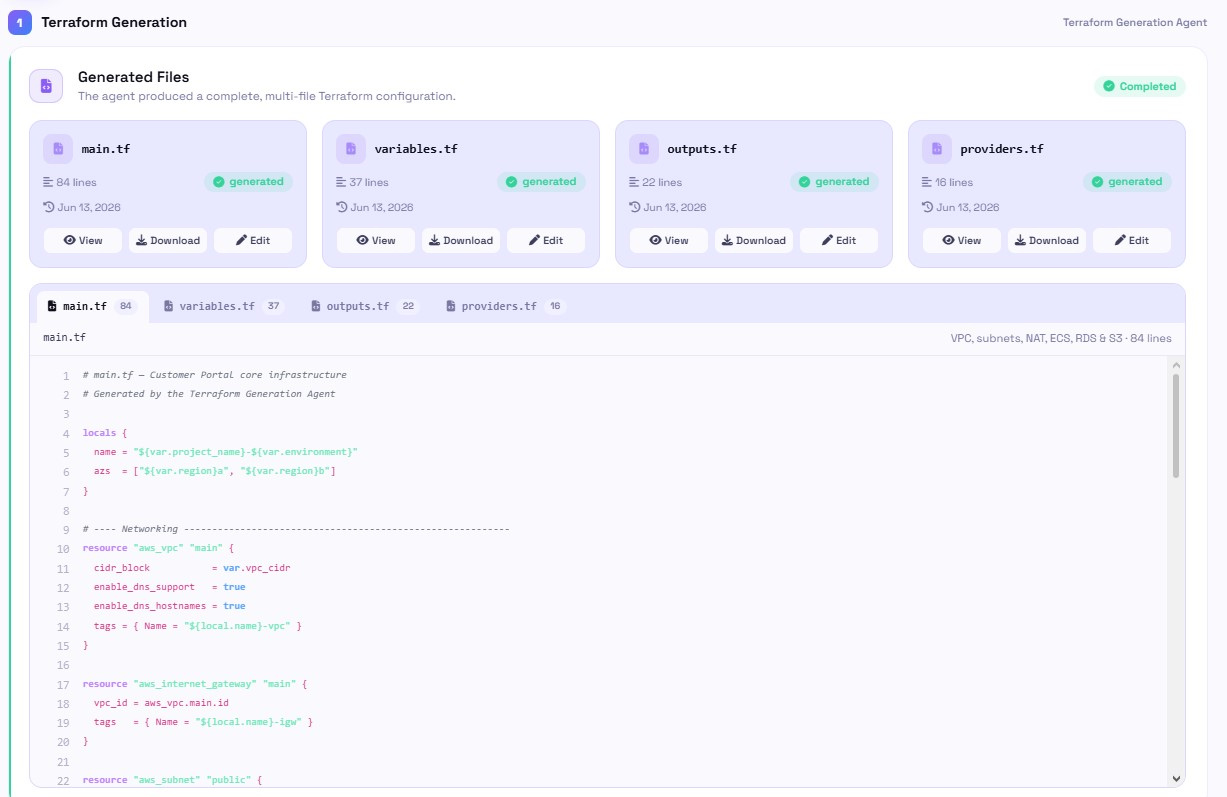
\includegraphics[width=0.9\textwidth]{images/TF Generation.jpg}
    \caption{Génération des fichiers Terraform}
    \label{fig:tf-generation}
\end{figure}

La figure~\ref{fig:tf-generation} montre la génération des fichiers Terraform
correspondant à l'architecture retenue, dans le respect des conventions HCL.

\begin{figure}[H]
    \centering
    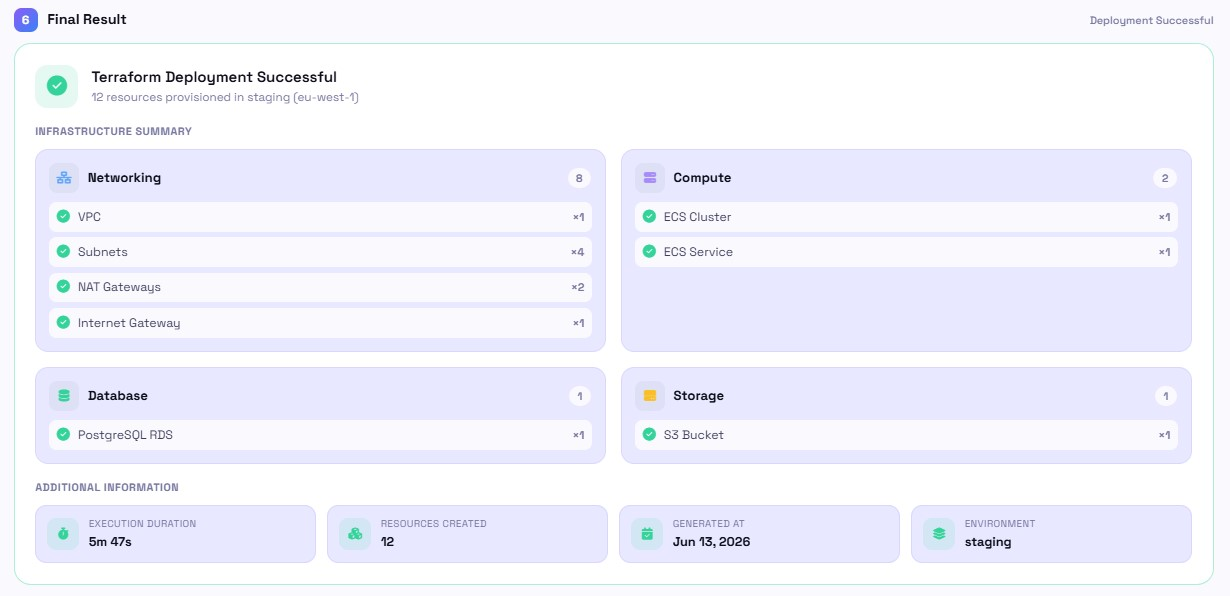
\includegraphics[width=0.9\textwidth]{images/final tf result.jpg}
    \caption{Résultat final de la génération Terraform}
    \label{fig:tf-final}
\end{figure}

La figure~\ref{fig:tf-final} présente les fichiers Terraform finalisés. Les ressources
déclarées sont cohérentes et prêtes à être validées puis planifiées.

\begin{figure}[H]
    \centering
    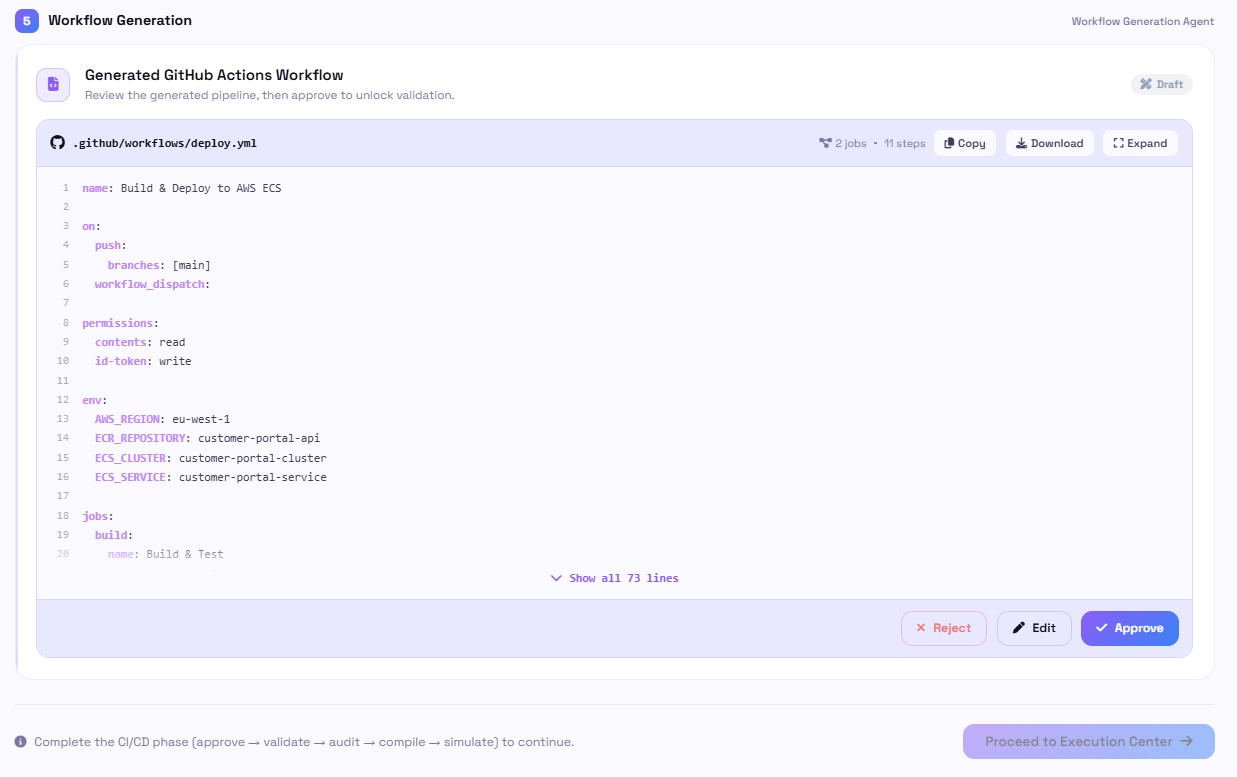
\includegraphics[width=0.9\textwidth]{images/Generated Github Action workflow.jpg}
    \caption{Workflow GitHub Actions généré}
    \label{fig:github-action}
\end{figure}

La figure~\ref{fig:github-action} illustre le pipeline GitHub Actions généré
automatiquement, intégrant les étapes de build, de test et de déploiement.

\subsection{Remédiation intelligente des erreurs}

En cas d'échec, le \textit{Corrector Agent} diagnostique l'erreur et propose une
correction soumise à la validation de l'utilisateur.

\begin{figure}[H]
    \centering
    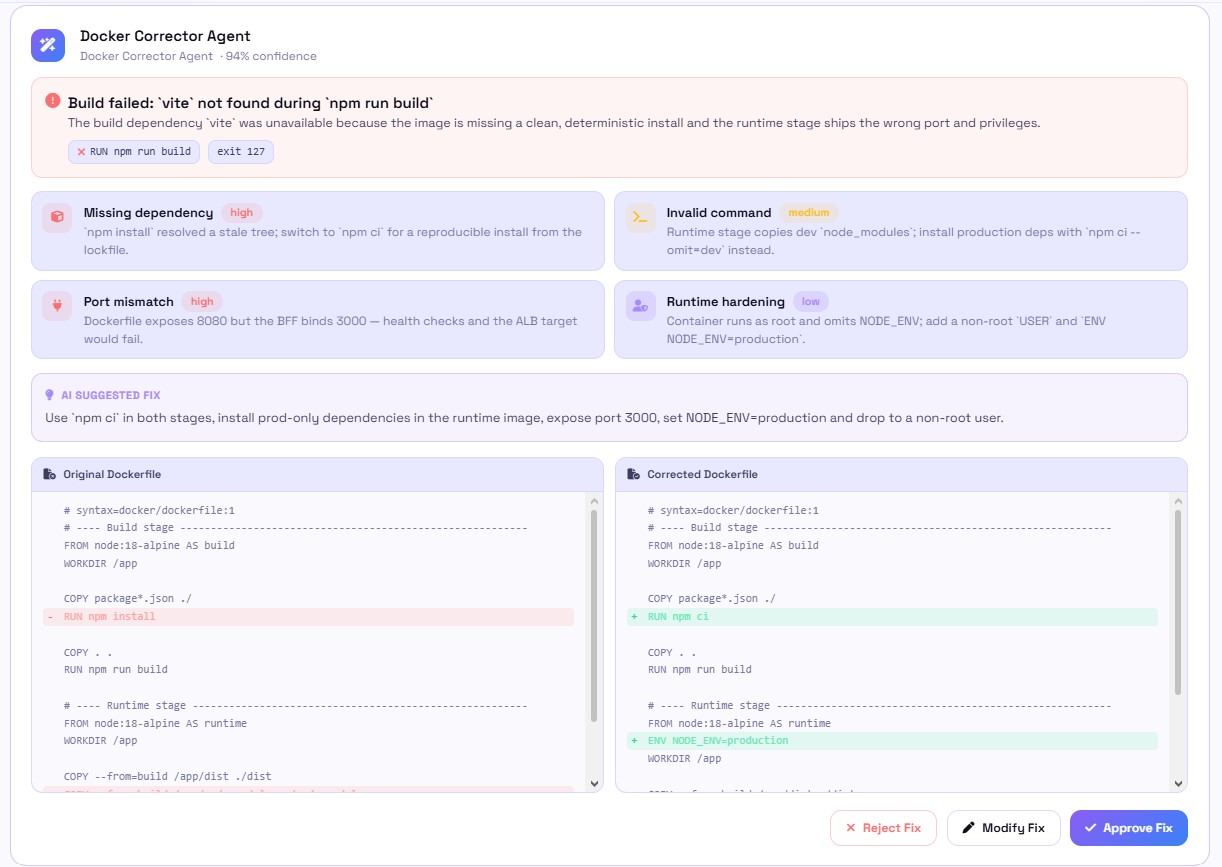
\includegraphics[width=0.9\textwidth]{images/Docker corrector agent.jpg}
    \caption{Correction assistée d'un Dockerfile}
    \label{fig:docker-corrector}
\end{figure}

La figure~\ref{fig:docker-corrector} montre le \textit{Corrector Agent} en action. À la
suite d'un échec de build, il analyse les journaux et propose une correction ciblée.

\begin{figure}[H]
    \centering
    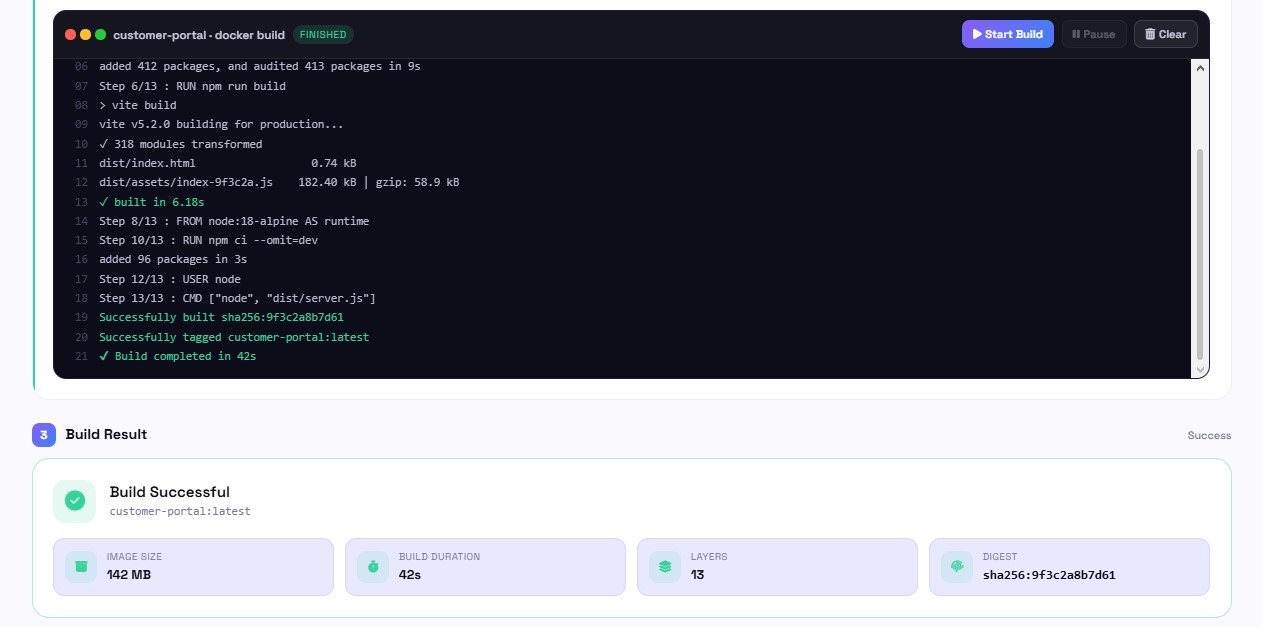
\includegraphics[width=0.9\textwidth]{images/Successfull docker build.jpg}
    \caption{Build Docker réussi après correction}
    \label{fig:docker-build-success}
\end{figure}

La figure~\ref{fig:docker-build-success} présente le résultat d'un build réussi après
application de la correction proposée, confirmant l'efficacité de la boucle de
remédiation.

\subsection{Validation et exécution des workflows}

La plateforme valide et exécute les artefacts générés tout en vérifiant leur conformité
et le respect des bonnes pratiques.

\begin{figure}[H]
    \centering
    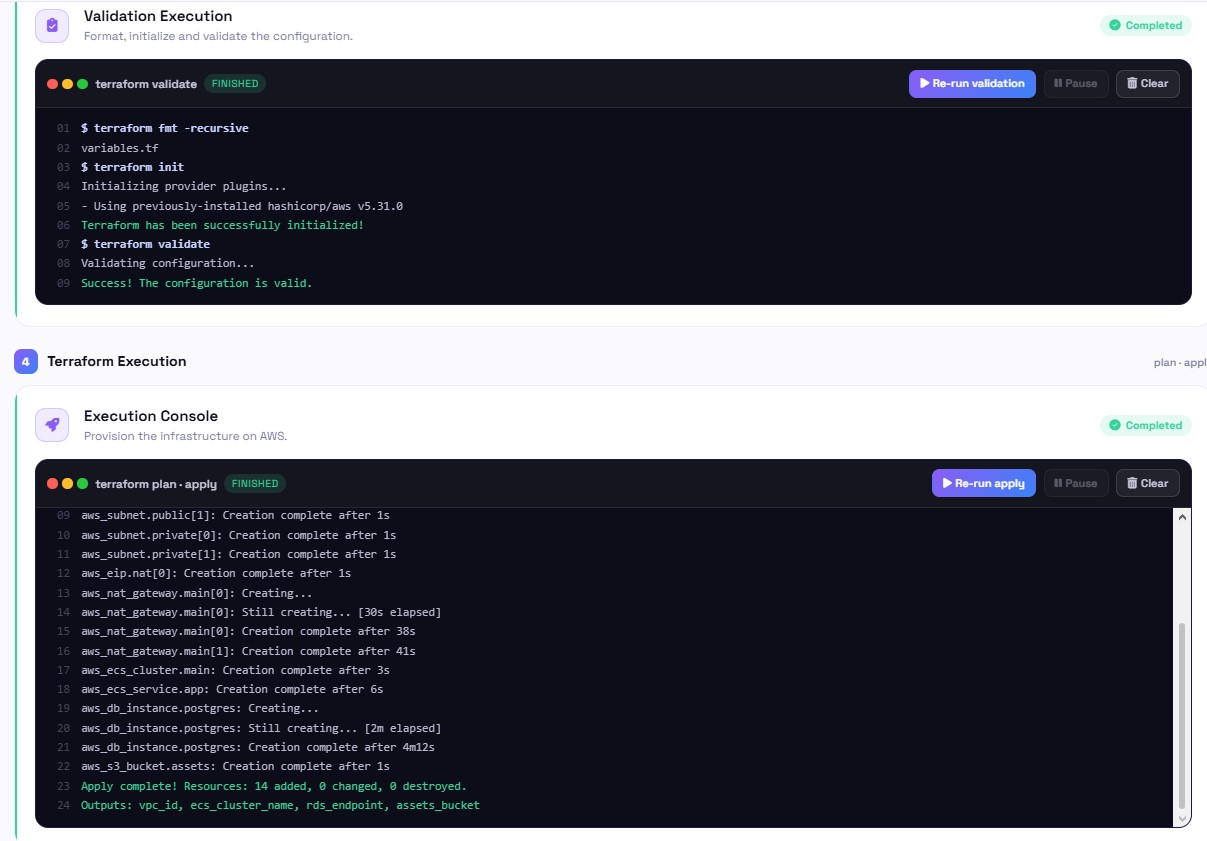
\includegraphics[width=0.9\textwidth]{images/tf execution success.jpg}
    \caption{Exécution Terraform réussie}
    \label{fig:tf-execution}
\end{figure}

La figure~\ref{fig:tf-execution} montre l'exécution réussie d'un plan Terraform. Les
ressources cloud sont provisionnées conformément à l'architecture sélectionnée.

\begin{figure}[H]
    \centering
    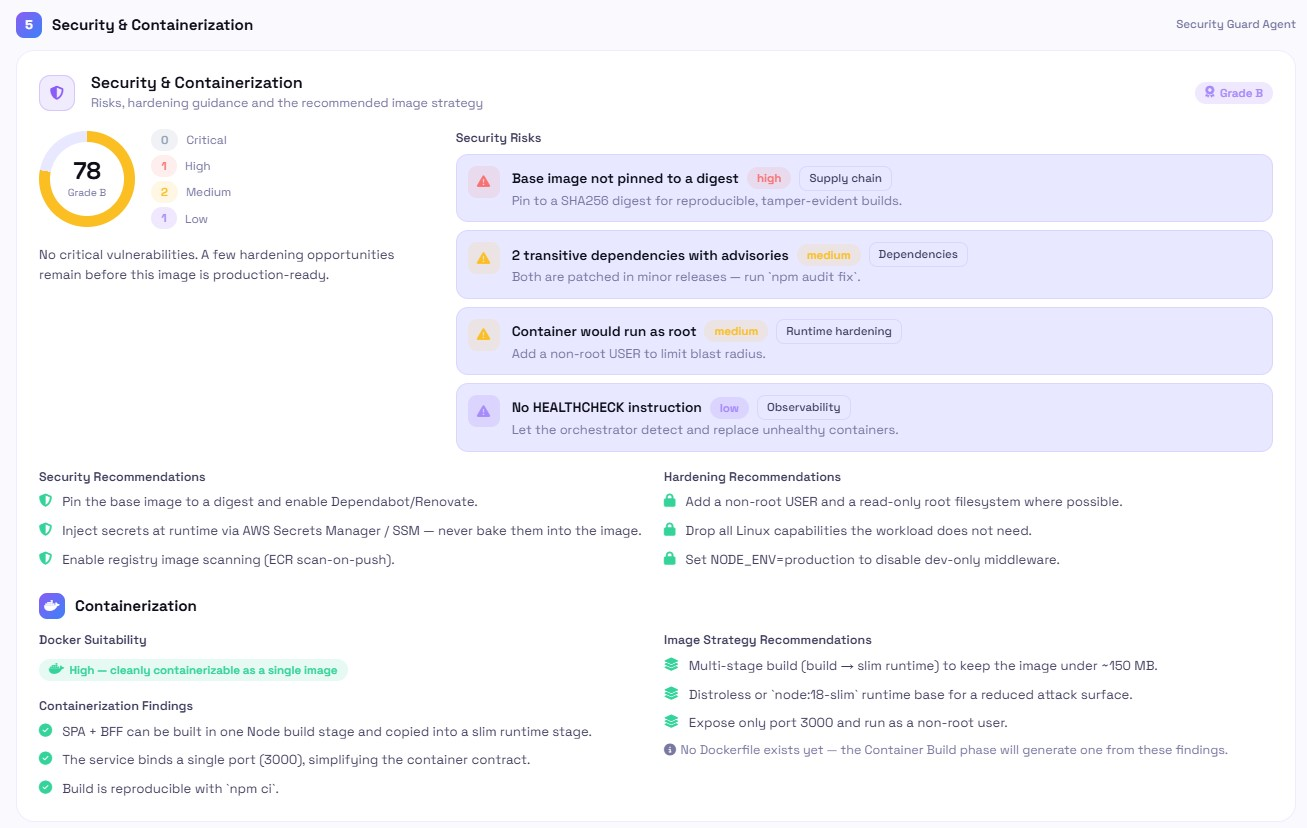
\includegraphics[width=0.9\textwidth]{images/Security agent.jpg}
    \caption{Vérification des bonnes pratiques dans les artefacts générés}
    \label{fig:security-agent}
\end{figure}

La figure~\ref{fig:security-agent} illustre la vérification des bonnes pratiques appliquée
aux artefacts générés. La sécurité y est traitée comme une exigence de qualité
transversale~: le contrôle vérifie que les artefacts respectent les bonnes pratiques
(utilisateur non-\textit{root}, permissions minimales, absence de secrets en clair) dès
leur génération, sans constituer une étape de sécurité isolée.

\section{Conclusion}

Ce chapitre a présenté la réalisation concrète de la plateforme. Nous avons d'abord
détaillé l'environnement de développement et les technologies retenues, puis illustré les
principales interfaces homme-machine couvrant l'authentification, la gestion des projets,
la sélection d'architecture et la génération des artefacts DevOps. Nous avons enfin validé
les capacités intelligentes du système~: la génération d'infrastructure cloud,
l'automatisation des pipelines CI/CD et la remédiation intelligente des erreurs.
L'ensemble confirme que la solution réalisée répond aux besoins exprimés et met
effectivement en œuvre les choix de conception définis précédemment.


    % --- Conclusion --------------------------------------------------
    \chapter*{CONCLUSION ET PERSPECTIVES}
\markboth{\MakeUppercase{CONCLUSION GÉNÉRALE}}{}
\addcontentsline{toc}{chapter}{CONCLUSION GÉNÉRALE}
\adjustmtc
\thispagestyle{MyStyle}

L'essor du Cloud Computing et des pratiques DevOps a considérablement élargi les
possibilités offertes aux équipes de développement, mais au prix d'une complexité
croissante~: multiplication des technologies à maîtriser, décisions d'architecture
nombreuses et préparation fastidieuse des artefacts de déploiement. C'est dans ce contexte
que s'inscrit ce projet de fin d'études, réalisé au sein de Talan Tunisie Consulting, dont
l'objectif était de concevoir une plateforme capable d'accompagner les ingénieurs Cloud et
DevOps tout au long de ce processus. La solution proposée, \textbf{MultiMindOps}, se
présente comme une plateforme d'assistance fondée sur l'intelligence artificielle~: elle
automatise les tâches répétitives de conception et de préparation de l'infrastructure, tout
en laissant à l'ingénieur la maîtrise des décisions stratégiques.

Au terme de ce travail, la plateforme réunit un ensemble de contributions cohérentes qui,
mises bout à bout, couvrent l'essentiel du cycle d'ingénierie Cloud. À partir d'une simple
analyse automatique d'un projet, MultiMindOps recommande plusieurs architectures cloud
accompagnées d'une estimation des coûts, puis génère de façon cohérente les principaux
artefacts DevOps~--- Docker, Terraform et pipelines GitHub Actions. Sa valeur ne tient pas
seulement à cette automatisation, mais à la fiabilité qu'elle apporte~: une boucle de
remédiation intelligente diagnostique et corrige les erreurs d'exécution, tandis qu'une
logique \textit{Human-in-the-Loop} soumet chaque décision critique à la validation de
l'ingénieur. La sécurité y est traitée comme une exigence de qualité transversale, intégrée
aux artefacts générés plutôt que comme une étape isolée. La plateforme réduit ainsi la
charge cognitive et le temps de mise en place d'une infrastructure cloud, sans jamais
dessaisir l'humain de son rôle de décideur.

\section*{Perspectives}
\addcontentsline{toc}{section}{Perspectives}

Plusieurs pistes réalistes prolongent ce travail. À court terme, l'optimisation du temps
d'exécution des workflows et l'amélioration continue des recommandations grâce aux retours
des utilisateurs renforceraient l'expérience d'usage. À moyen terme, l'extension de la
plateforme à d'autres fournisseurs cloud, tels qu'Azure et Google Cloud Platform,
élargirait son champ d'application au-delà d'AWS. Enfin, l'enrichissement progressif de la
base de connaissances RAG et l'ajout de nouveaux agents spécialisés permettraient de couvrir
davantage de types d'artefacts et de cas d'usage, tout en préservant la cohérence de
l'architecture multi-agents existante.


    % --- Bibliographie / Webographie ---------------------------------
    \addcontentsline{toc}{chapter}{WEBOGRAPHIE}

\adjustmtc
\renewcommand\bibname{WEBOGRAPHIE}

\begin{thebibliography}{9}

\bibitem{TALAN}
\textbf{Talan Tunisie}. Page web de l'entreprise \textbf{[en ligne]}.\\Dernière consultation : 21/03/2025.\\Disponible à : \url{https://www.talan.com/global/fr}

\bibitem{NIST_CLOUD}
P. Mell, T. Grance. \textbf{The NIST Definition of Cloud Computing}. NIST Special
Publication 800-145, National Institute of Standards and Technology, 2011.

\bibitem{CNCF}
\textbf{Cloud Native Computing Foundation}. CNCF Cloud Native Definition v1.0
\textbf{[en ligne]}.\\Dernière consultation : 05/07/2026.\\Disponible à :
\url{https://github.com/cncf/toc/blob/main/DEFINITION.md}

\bibitem{IAC_MORRIS}
K. Morris. \textbf{Infrastructure as Code: Dynamic Systems for the Cloud Age}. 2\textsuperscript{e}
édition, O'Reilly Media, 2020.

\bibitem{DEVOPS_HANDBOOK}
G. Kim, J. Humble, P. Debois, J. Willis. \textbf{The DevOps Handbook}. IT Revolution
Press, 2016.

\bibitem{HARNESS_AIDA}
\textbf{Harness}. AI-Driven DevOps Assistant (AIDA) \textbf{[en ligne]}.\\Dernière
consultation : 05/07/2026.\\Disponible à : \url{https://www.harness.io}

\bibitem{PULUMI_INSIGHTS}
\textbf{Pulumi}. Pulumi Insights \textbf{[en ligne]}.\\Dernière consultation :
05/07/2026.\\Disponible à : \url{https://www.pulumi.com/product/insights/}

\bibitem{CLAUDE_CODE}
\textbf{Anthropic}. Claude Code \textbf{[en ligne]}.\\Dernière consultation :
05/07/2026.\\Disponible à : \url{https://www.anthropic.com/claude-code}

\bibitem{AWS_WELL_ARCHITECTED}
\textbf{Amazon Web Services}. AWS Well-Architected Framework \textbf{[en ligne]}.\\Dernière
consultation : 05/07/2026.\\Disponible à :
\url{https://aws.amazon.com/architecture/well-architected/}

\bibitem{TERRAFORM_DOCS}
\textbf{HashiCorp}. Terraform Documentation \textbf{[en ligne]}.\\Dernière consultation :
05/07/2026.\\Disponible à : \url{https://developer.hashicorp.com/terraform/docs}

\bibitem{DOCKER_DOCS}
\textbf{Docker Inc.} Docker Documentation \textbf{[en ligne]}.\\Dernière consultation :
05/07/2026.\\Disponible à : \url{https://docs.docker.com}

\bibitem{K8S_DOCS}
\textbf{The Kubernetes Authors}. Kubernetes Documentation \textbf{[en ligne]}.\\Dernière
consultation : 05/07/2026.\\Disponible à : \url{https://kubernetes.io/docs/}

\bibitem{GITHUB_ACTIONS_DOCS}
\textbf{GitHub}. GitHub Actions Documentation \textbf{[en ligne]}.\\Dernière consultation :
05/07/2026.\\Disponible à : \url{https://docs.github.com/en/actions}

\bibitem{OPENAI_DOCS}
\textbf{OpenAI}. OpenAI Platform Documentation \textbf{[en ligne]}.\\Dernière consultation :
05/07/2026.\\Disponible à : \url{https://platform.openai.com/docs}

\bibitem{LANGGRAPH}
\textbf{LangChain}. LangGraph Documentation \textbf{[en ligne]}.\\Dernière consultation :
05/07/2026.\\Disponible à : \url{https://langchain-ai.github.io/langgraph/}

\bibitem{RAG_LEWIS}
P. Lewis, E. Perez, A. Piktus, \textit{et al.} \textbf{Retrieval-Augmented Generation for
Knowledge-Intensive NLP Tasks}. Advances in Neural Information Processing Systems (NeurIPS),
2020.

\bibitem{HITL_MOSQUEIRA}
E. Mosqueira-Rey, E. Hernández-Pereira, D. Alonso-Ríos, \textit{et al.} \textbf{Human-in-the-loop
machine learning: a state of the art}. Artificial Intelligence Review, vol. 56, 2023.


\end{thebibliography}


    % Annexes : décommentez la ligne suivante APRÈS avoir ajouté l'image
    % référencée (images/your_image.png) — voir le rapport de diagnostic.
    % \chapter*{ANNEXES}
\markboth{\MakeUppercase{ANNEXES}}{}
\addcontentsline{toc}{chapter}{ANNEXES}
\adjustmtc
\thispagestyle{MyStyle}

%% add to table of contents : Annexe.1
\makeatletter\renewcommand\thesection{A.\@arabic\c@section}\makeatother

%add spacing in the table of figures
\addtocontents{lof}{\vspace{0.3cm}}

\appendix
\renewcommand{\thefigure}{A.\arabic{figure}}
\setcounter{figure}{0}
\section{TITRE ANNEXE 1}
Lorem ipsum dolor sit amet, consectetur adipiscing elit. Sed non risus. Suspendisse lectus tortor, dignissim sit amet, adipiscing nec, ultricies sed, dolor. Cras elementum ultrices diam. Maecenas ligula massa, varius a, semper congue, euismod non, mi. Proin porttitor, orci nec nonummy molestie, enim est eleifend mi, non fermentum diam nisl sit amet erat. Duis semper. Duis arcu massa, scelerisque vitae, consequat in, pretium a, enim.\par
\begin{figure}[H]%
    \center%
    \setlength{\fboxsep}{5pt}%
    \setlength{\fboxrule}{0.5pt}%
    \fbox{
    \includegraphics[width=6.5cm,height=9cm]{images/your_image.png}%
    }
    \caption{Titre de figure annexe 1}%
\end{figure}

\section{TITRE ANNEXE 2}
Lorem ipsum dolor sit amet, consectetur adipiscing elit. Sed non risus. Suspendisse lectus tortor, dignissim sit amet, adipiscing nec, ultricies sed, dolor. Cras elementum ultrices diam. Maecenas ligula massa, varius a, semper congue, euismod non, mi. Proin porttitor, orci nec nonummy molestie, enim est eleifend mi, non fermentum diam nisl sit amet erat. Duis semper. Duis arcu massa, scelerisque vitae, consequat in, pretium a, enim. Pellentesque congue. Ut in risus volutpat libero pharetra tempor.\par
\begin{figure}[H]%
    \center%
    \setlength{\fboxsep}{5pt}%
    \setlength{\fboxrule}{0.5pt}%
    \fbox{
    \includegraphics[width=6.5cm,height=9cm]{images/your_image.png}%
    }
    \caption{Titre de figure annexe 2}%
\end{figure}


\end{document}
